% !TEX root = ../thesis-example.tex
%
\chapter{L'instrument et le geste}
\label{ch:gesture}

\cleanchapterquote{La percussion de ce pseudo-gong est illlusoire :\\
rien ne tape sur rien dans l’ordinateur.\\
Schumann qualifiait le legato au piano\\
de ``trompe-l’oreille'' : la musique est aussi un art\\
du mirage, de l’illusion.}{Jean-Claude Risset}{Discours invité aux JIM 2010 \cite{risset_propos_2010}}

%L'expression musicale a été contrainte (et non ``prisonnière'', car la contrainte peut être fertile) par la relation causale entre le geste d'excitation et le son produit par l'instrument dans les lutheries acoustiques.

\vspace*{\fill}

\noindent Poursuivant des évolutions organologiques latentes, telles que présentées dans la section \ref{sec:ephemerality:landscape}, les \glspl{DMI} finissent d'opérer un découplage énergétique, une ``dislocation du contrôle'' (\textit{control dislocation} \cite{miranda_new_2006}), rompant avec plus de 35.000 ans de tradition musicale \cite{conard_new_2009} et avec l'unité de temps, de lieu et d'action —définie en règle par le théâtre classique, mais qui reflète la relation qui existait entre l'auditeur et le phénomène sonore, comme le rappelle Hugues Genevois dans \cite{cance_what_2012}.\\
\indent L'introduction de la mémoire et de la computation numérique permet une re-programmation complète de l'interaction, rendant leur fonctionnement à la fois complexe et cryptique. Cet aspect peut se révéler être un inconvénient, dans la mesure où il prive le public d’une lecture possible de la performance musicale. Cela peut cependant s’avérer être un avantage, si l'on considère que la performance musicale comporte une part scénographique dans laquelle l’illusion a toute sa place.\\
\indent Nous allons voir dans ce chapitre comment le geste instrumental s'en trouve affecté, par un examen critique des catégories gestuelles déjà proposées, la proposition de nouvelles catégories prenant en compte l'aspect subversif de l'art musical et les conséquences que nous pouvons en tirer en termes de conceptions des \glspl{DMI}.

\clearpage

\section{Introduction : L'étude du geste en musique}

\noindent Si l'étude du rythme et plus encore, des hauteurs, a été particulièrement importante dans la culture classique occidentale, l'étude du geste a longtemps été négligée voire méprisée, comme le rapporte Jean-Marc Warszawski\footnote{Texte publié d'après la conférence ``La musique et le geste'' en octobre 2012, disponible en ligne : \url{https://www.musicologie.org/18/la_musique_et_le_geste.html}.}: \iquote{La tradition savante occidentale, grâce à l'écriture, dématérialise le geste créatif musicien, et impose une ligne de démarcation ente musique écrite et non écrite, en quelque sorte une frontière entre le primitif et le civilisé.}\\
\indent Peut-être faut-il également y voir une autre raison : le geste ne se laisse pas aussi facilement mesurer, encore moins définir, que la hauteur. Si cette dernière peut se  réduire en première approximation à une grandeur physique mesurable --~sa fréquence fondamentale\footnote{La perception de la hauteur est évidemment plus complexe que l'évalutation de la fondamentale et un des sujets d'étude de la psycho-acoustique, voir notamment les travaux de Michèle Castellengo \cite{castellengo_ecoute_2015}. L'écriture musicale classique s'est toutefois largement construite sur cette réduction, que Robert Francès nomme ``abstraction notale'' \cite{frances_perception_1984}.}, le geste ne se laisse pas aussi facilement réduire à une mesure. Il entraine depuis sa production jusqu'à sa réception toute la complexité du vivant : sa multidimensionalité, son instabilité, sa relativité, sa combinatoire, et l'ensemble de ses aspects culturels... (TODO : développer et/ou enlever les pointillés)\\
\indent L'étude du geste se développe dans le courant du \siecle{19}~siècle, sous l'effet de la révolution industrielle, de l'étude mécanique du mouvement et la création de conservatoires qui développent des techniques d'apprentissage où le geste est pris en compte\footnote{Voir en particulier la collection rassemblée sur le site de la Bibliothèque Nationale de France: \url{https://gallica.bnf.fr/html/und/partitions/oeuvres-theoriques-et-pedagogiques}. L'intérêt pour le geste à cette période de développement industriel donne lieu par ailleurs à l'invention d'étonnants systèmes mécaniques servant à guider, contraindre et fortifier les gestes, en particulier pour le piano, tels que le ``chiroplaste'' ou le ``dactylion'', mais qui s'avèrent être davantage des instruments de torture, endommageant parfois les mains de manière irréversible.}. L'étude du geste a progressivement gagné en importance, d'une part avec l'émergence de l'anthropologie au début du \siecle{20}~siècle, et d'autre part suite à l'explosion des technologies de télécommunication, lorsque sa compréhension et sa modélisation sont devenues nécessaires pour le développement des \gls{IHM} dans la seconde moitié du siècle, jusqu'à devenir un domaine d'étude à part entière, les \textit{gesture studies}, soutenue notamment par l'\gls{ISGS} créée en 2002.\\
\indent Dans le domaine de la musique, c'est l'arrivée du ``temps-réel'' et l'émergence des \glspl{DMI} dans les années 1980, qui entraine la parution croissante d'articles traitant de la question du geste instrumental. Au tournant du siècle (du millénaire), le geste devient un objet d'étude majeur dans le domaine de l'informatique musicale, se traduisant notamment par la parution d'ouvrages collectifs dédiés\footnote{Voir en particulier : \cite{genevois_les_1999}, \cite{wanderley_trends_2000} et \cite{godoy_musical_2010}}, ainsi par que l'apparition de la conférence \gls{NIME} en 2001, qui lui accorde une place importante.\\
\indent Plusieurs projets de recherche interdisciplinaires ont également été menés, comme le projet ConGAS\footnote{``Gesture Controlled Audio Systems'', projet financé entre 2003 et 2007 dans le cadre de la Coopération Européenne en Sciences et Technologies (COST Action 287)}, ou plus récemment le projet Gemme\footnote{``Geste musical : modèles et expériences'', projet de recherche financé par l'ANR de 2012 à 2016, dont un carnet de recherche en ligne est disponible : \url{https://geste.hypotheses.org/gemme}} et la chaire thématique pluridisciplinaire GeAcMus\footnote{La chaire``Geste - Acoustique - Musique'' a été créée en 2015 à Sorbonne Université \url{http://www.sorbonne-universites.fr/actions/recherche/chaires-thematiques/geacmus.html}} créée à Sorbonne-Université.

\extra{Le terme Gesture est utilisé dans 62\% des articles publiés à NIME (cf. Jensenius paper : To Gesture or Not? An Analysis of Terminology in NIME Proceedings 2001–2013) <= update this}

%%%%%%%%%%%%%%%%%%%%%%%%%%%%%%%%%%%%%%%%%%%%%%%%%%%%%%%%
\section{Geste instrumental et geste musical}

\subsection{La musique et ses instruments}

\noindent La définition du geste musical pose le double problème de définir ce qu'on entend par ``geste'' et par ``musique''. Pour ce qui est de la musique, j'adopterai ici la définition proposée par Christopher Small, non pas du \textit{nom} ``musique'', mais du \textit{verbe} qu'il invente : ``musiquer'' \cite{small_musicking:_1998}:
\iquote{Musiquer, c'est participer, à quelque titre que ce soit, à une performance musicale, que ce soit en jouant, en écoutant, en répétant ou en pratiquant, en fournissant du matériel pour la performance (ce qu'on appelle ``composer''), ou en dansant. Nous pourrions même parfois en étendre le sens à ce que font la personne qui prend les billets à l'entrée, les gros bras qui déplacent le piano et les tambours, les roadies qui installent les instruments et font les balances ou les personnes qui nettoient après que tout le monde soit parti. Ils contribuent tous, eux aussi, à la nature de l'événement qu'est une performance musicale.}\\
\indent Si j'adopte ce néologisme, ce n'est pas pour l'exhaustivité que semble conférer une définition aussi large mais essentiellement pour deux raisons: la première est le choix d'utiliser un verbe plutôt qu'un nom, c'est-à-dire d'identifier une pratique plutôt qu'un objet, ce qui dans le cas de la performance musicale semble mieux adapté. La deuxième raison est liée au contexte technico-culturel dans lequel ces pratiques s'inscrivent: la reconfiguration des modes de production et de réception de la musique\footnote{voir à ce sujet l'ouvrage de Paul Théberge \cite{theberge_any_1997}} qu'ont entrainée les évolutions technologiques du \siecle{20}~siècle ont rendu poreuses les frontières entre les différentes pratiques liées à la création musicale. Je restreindrai toutefois le champ de cette définition aux pratiques qui gravitent directement autour de l'instrument de musique, tel que présenté dans le chapitre précédent.\\
\indent Partant de cette définition et reprenant une proposition d'Hugues Genevois \cite{genevois_geste_1999}, on peut distinguer plusieurs phases au cours desquelles se manifeste un geste musical :
%---------------------
\vspace{-1em}
\begin{itemize}[noitemsep]
\item \textbf{la composition} : la production de structure musicales hors-temps de leur rendu sonore;
\item \textbf{la lutherie} : la réalisation de l'instrument et sa préparation pour le jeu;
\item \textbf{la performance} : le jeu instrumental qui produit, modifie, mélange, dans le temps même de l'écoute, la matière sonore, les gestes de l'instrumentiste, du chef, de l'ingénieur du son;
\item \textbf{l'écoute} : qui construit l'intelligibilité de notre environnement sonore et se mobilise sans répit pour en garantir la cohérence;
\item \textbf{la pédagogie} : durant laquelle la complexité du geste musical se transmet progressivement, en étant guidée, soutenue, encouragée, critiquée, en se pratiquant parfois sous la forme d'exercices idiomatiques et systématiques (e.g. faire ses gammes), et à travers des allers-retours entre performance et écoute.
\end{itemize}
%---------------------
\noindent La ``geste'' en musique a été utilisée pour décrire différents aspects de la relation qu'entretiennent le mouvement, l'instrument, l'intention, la morphologie et la signification du son ou encore les formes d'écritures compositionnelles. L'instrument de musique se trouvant à la croisée de ces différents chemins, la notion de ``geste instrumental'' a souvent été liée voire confondue avec celle de ``geste musical''. Dans la pratique, ces différents gestes se superposent souvent mais pourront se traduire par différentes formes de configurations instrumentales, adaptées aux spécificités de chaque situation.

\subsection{Aspects du geste}

\noindent Dans sa définition générale, le Littré, le Larousse ou le dictionnaire de l'Académie Française s'accordent à le définir comme \iquote{un mouvement du corps, principalement de la main, des bras, de la tête, porteur de sens ou non} (Larousse).

\subsubsection{Aspects phénoménologiques}

\noindent Un premier aspect du geste est sa nature de mouvement, son déploiement spatial et temporel, dont les qualités spatiales, cinématiques, cinétiques, synchroniques, fréquentielles, balistiques (...) abstraites font écho à la mémoire de tous les mouvements dont nous faisons l'expérience: battements, ondulations, chutes, éclosions, envols, éruptions, roulements, contractions, extensions, sursauts... Le geste possède une force expressive, en dehors de toute interprétation sémiotique, génératrice de sensations dont la logique ne peut être décrite que par la métaphore\footnote{C'est en particulier l'entreprise de Gaston Bachelard dans son travail de ``phénoménologie de l'imagination'', dont ``L'air et les Songes, Essai sur l'imagination du mouvement''\cite{bachelard_air_1943}}.\\
\indent Ce mouvement est l'expression même du vivant et il reflète à la fois la relation du corps à son environnement externe (force de gravité et cinétique, contournement d'obstacles, frictions sur les matériaux, contraintes formelles chorégraphiques...) et l'expression des mouvements internes du corps (vigueur ou mollesse, souple ou crispé, émotion se traduisant par des gestes tels que haussement d'épaule, sursaut de surprise, grimaces diverses, etc.). La maitrise de ces mouvements est un aspect fondamental de la danse qui, comme la musique le fait avec le son, met en œuvre le corps dans des intensités, des rythmes, des trajectoires. Si les gestes de la danse ne sont pas \textit{a priori} instrumentaux, les \glspl{DMI} rendent plus que jamais possible leur utilisation à des fins d'interaction musicale, comme nous le verrons plus loin (cf. notamment \cite{bevilacqua_gesture_2011, alaoui_movement_2012, silang_maranan_designing_2014, hsueh_understanding_2019}.)

\subsubsection{Aspects sémiotiques}

\noindent Un deuxième aspect du geste est indiqué par le curieux épithète de la définition précédente : ``porteur de sens ou non''. S'il a semblé utile d'évoquer une qualité potentiellement absente, c'est précisément parce les différentes définitions qu'on donne du geste dépendent en partie de cet aspect sémiotique, qui reste soumis à une interprétation subjective et contextuelle dans un système de valeurs. Les significations d'un geste peuvent en effet être attribuées par l'auteur du geste ou bien par celui ou celle qui observe ce geste, sans qu'il n'y ait nécessairement de correspondance, ni en terme de signification, ni sur la part du mouvement considérée signifiante. La signification d'un geste peut également être attribuée par la machine, en particulier dans les systèmes d'apprentissage, comme nous le verrons plus loin.\\
\indent Cependant, par rapport aux théories de la sémiologie du geste communicationnel développées notamment par David McNeil \cite{mcneill_gesture_2005} ou Adam Kendon \cite{kendon_gesture:_2004}, le geste musical semble davantage se situer à un niveau pré-sémiotique\footnote{Guerino Mazzola propose une analyse conséquente de cette aspect pré-sémiotique du geste dans le troisième volume de \textit{Topos of Music} \cite{mazzola_topos_2018}}, qui permet aux gestes de se déployer de manière créative en potentialisant de multiples significations\footnote{Merleau-Ponty résume élégamment cette force créative par la formule \iquote{La parole est un geste et sa signification un monde} dans \cite{merleau-ponty_phenomenologie_1976}} et permet leur interprétation esthésique\footnote{Jean-Jacques Nattiez développe une sémiologie de la musique qui s'appuie notamment sur les concepts d'analyse poiétique, concernant les processus de fabrication, et esthésique, concernant ceux de leur réception.} à de multiples niveaux.

\subsubsection{Aspects ergotiques}

\noindent Une autre définition du geste relève sa dimension manipulative : \iquote{Manière de mouvoir le corps, les membres et, en particulier, manière de mouvoir les mains dans un but de préhension, de manipulation} (Larousse). Cette définition met l'accent sur la relation possible entre le geste et un objet, un outil, un instrument et s'applique par conséquence particulièrement bien à la situation instrumentale. Un aspect qui lui est lié est la fonction épistémique du geste\footnote{La fonction épistémique sera par ailleurs évoquée dans le chapitre suivant, en ce qui concerne ses implications sur le design de l'interface de jeu.}, qui permet de se prendre connaissance de son environnement, des matériaux, de se situer et de s'ajuster en permanence. C'est sur ces aspects que se concentre notamment les typologies gestuelles proposées par Claude Cadoz que je discuterai plus loin.\\

\subsubsection{Aspects (dia)grammatiques}

\noindent Enfin, si le geste \textit{ex-prime} (du latin \textit{ex-premo} : ``faire sortir en pressant'') des mouvements internes du corps, il \textit{im-prime} et laisse une trace dans la matière, dans la machine, dans les esprits. C'est parfois cette trace résultante qu'on nomme geste, par métonymie et analogie avec les qualités de mouvement qui sont à son origine, lorsqu'on parle par exemple du \textit{geste de composition}. Les capacités des machines à enregistrer le geste dans sa dynamique --~auparavant éphémère et seulement visible sous la forme de traces statiques: littérature, peinture, partition~-- confèrent à cet aspect \textit{diagrammatique} du geste une importance particulière à l'époque de sa reproductibilité technique\footnote{L'expression utilisée ici revoie bien évidemment à l'œuvre éponyme de Walter Benjamin\cite{benjamin_loeuvre_2013}}, qui sera analysée à la lumière de la notion de (dia)gramme proposée par Gilles Deleuze et Bernard Stiegler.

%--------------------------------------------


% Jensenius in Musical Gesture : "Based on the above viewpoints, it seems straightforward to define musical gesture as an action pattern that produces music, is encoded in music, or is made in response to music. Qualifications can be added to the term musical gesture whenever needed to avoid misunderstandings. For example, one can speak about sound-producing gestures, sound-modifying gestures, sound-accompanying gestures, sonic gestures, playing gestures, and so on."

%-------------------------------------------
\subsection{Spécificités des DMIs}

\subsubsection{Les DMIs ne sont pas (que) des instruments acoustiques}

\noindent Dans le contexte particulier des lutheries numériques, un certain nombre de problèmes se posent par rapport au geste instrumental sur les instruments acoustiques, liés à des spécificités du numérique que nous avons déjà en partie évoqué dans le chapitre précédent\footnote{De manière plus globale et sociologique, les révolutions technologiques électroniques ont également modifiés les modes de production et de réception de la musique à l'échelle industrielle, entrainant d'autres conséquences que celles listées ci-après, mais qui dépassent le sujet que nous traitons ici. Je renvoie pour ces questions là au travail de TODO : Bacot, Collins, Auslander, Rebecca Bennett, etc.}.
%-----------
\vspace{-1em}
\begin{itemize}[noitemsep]
\item \textbf{le découplage énergétique} : ce découplage est la différence la plus saillante par rapport aux lutheries acoustiques. Certains de ses aspects sont déjà présents dans les instruments électriques et électroniques, mais l'informatique numérique ajoute un découplage de plus: les signaux (gestuels, sonores) n'y existent plus sous forme analogique et se présentent sous la forme de représentations numériques du signal, c'est-à-dire encodés dans un alphabet.
\item \textbf{la mémoire et le temps différé}: si le terme de ``temps réel'' est abondemment utilisé quand on parle des \glspl{DMI}, il ne faut pas oublier que l'informatique introduit avant tout le temps la possiblité du temps différé, de l'enregistrement exploitable dans le futur.
\item \textbf{la computation} : le traitement algorithmique permet --~ou impose~-- une reconfiguration permanente des modèles et des représentations, qui entraine une instabilité, un métamorphisme des relations entre les données.
\end{itemize}
%-----------
\noindent Par ailleurs, les \glspl{DMI} ne sont encore souvent pas considérés par les institutions musicales au même titre que les instruments acoustiques: leur pratique n'est pas enseignée en tant que telle dans les conservatoires\footnote{La pratique musicale des \gls{DMI} est généralement reléguée à une pratique optionnelle dans les classes de composition électroacoustique ou \gls{MAO}}, et la partie électronique dans les concerts institutionnels est souvent absente de la scène\footnote{C'est particulièrement le cas pour les concerts de musique mixte dans la tradition de l'\gls{IRCAM}, beaucoup moins pour les concerts organisés par le \gls{GRM} dont l'histoire n'a pas cet ancrage dans la musique classique acoustique.} et confiée à un \gls{RIM} (et non à un ``musicien'') au statut ambigu\footnote{Voir notamment l'analyse de Laura Zattra sur l'origine du statut de \gls{RIM} à l'\gls{IRCAM}: \cite{zattra_les_2013}} et qui opère généralement dans l'ombre. Cette situation n'a guère favorisé la considération des interfaces électroniques et des nouveaux gestes qui leur étaient propres en tant qu'instruments de performance musicale à part entière.

%-------------------------------------------
\subsubsection{Les DMIs ne sont pas des ``interfaces utilisateur''}

\noindent Un biais de l'approche fonctionnelle des \gls{IHM} est lié au fait que l'interaction a longtemps été définie (et l'est parfois encore) par la perspective d'une tâche que l'utilisateur doit accomplir. Ce contexte écologique a contribué au développement de tout un champ d'étude dans le domaine des \gls{IHM}: les \textit{user studies}, transposé dans le domaine de l'ingénierie industrielle sous le nom d'``Experience Utilisateur''\footnote{En abrégé : UX pour User eXperience; le métier de ``UX designer'' étant désormais très répandu dans le domaine du développement logiciel mais également appliqué à d'autres domaines tels que la grande consommation.}. L'efficacité dans l'accomplissement d'une tâche et l'absence d'effort qui constitue \iquote{une vertu cardinale dans la mythologie de l'ordinateur}\footnote{\iquote{Most computer instruments in use are those provided by the commercial music industry. Their inadequacy has been obvious from the start; emphasizing rather than narrowing the separation of the musician from the sound. Too often controllers are selected to minimize the physical, selected because they are effortless. Effortlessness in fact is one of the cardinal virtues in the mythology of the computer.}dans \cite{ryan_remarks_1991}} comme le notait Joel Ryan, ont longtemps été les principales motivation ayant guidé l'interaction dans les \gls{IHM}. La notion d'expérience utilisateur est venue étendre leur analyse éco-systémique en intégrant des aspects ésthétiques ou émotionnels dans leur design, mais qui privilégie généralement la recherche d'une utilisation facile et confortable pour l'utilisateur.\\
%---- Figure : instruments abusers---------
\begin{figure}[!htbp]
	\captionsetup{format=plain}%
	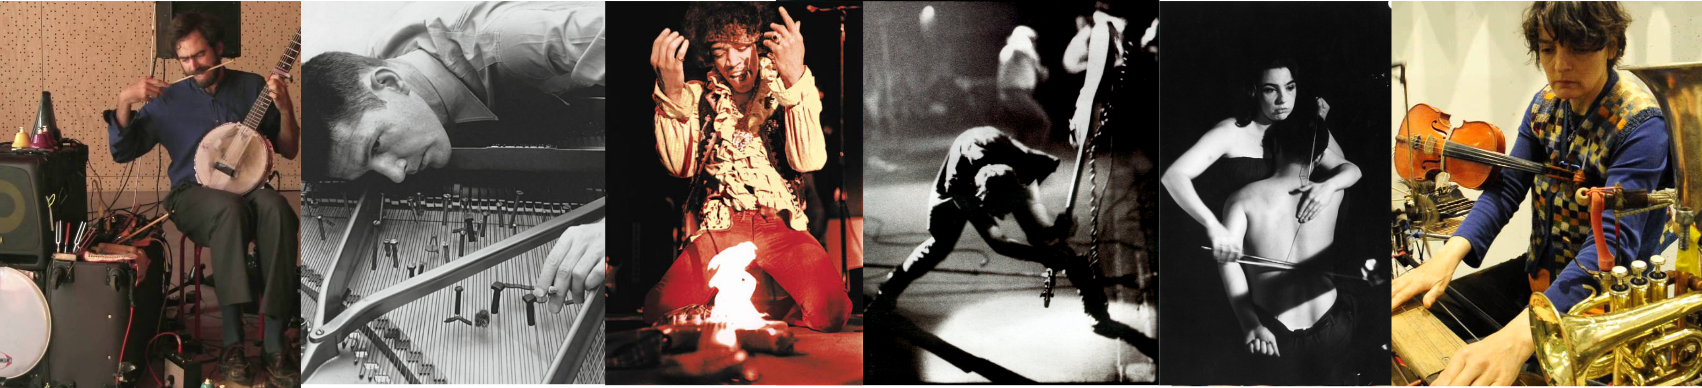
\includegraphics[width=\textwidth]{gfx/03_gesture/instrumentabusers.png}
	\caption[Les instrument ne sont pas des interfaces utilisateur]{Les instrument ne sont pas des interfaces utilisateur. De gauche à droite : Thomas Bonvallet, John Cage, Jimi Hendrix, Paul Simonon, Charlotte Moorman, Sarah Kenchington}
	\label{fig:gesture:abusers}
\end{figure}
%---- Figure : instruments abusers---------
\indent Or dans une performance musicale vivante, cette situation n'existe pas. Le musicien ne saurait être défini comme ``l'utilisateur de son instrument''(figure \ref{fig:gesture:abusers}), pas plus que son instrument comme une ``interface utilisateur'', et comme le note Ryan, il serait tout aussi intéressant de rendre son contrôle aussi difficile que possible\footnote{\iquote{In designing a new instrument it might be just as interesting to make control as difficult as possible.} \cite{ryan_remarks_1991}}.Les musiciens cherchent bien souvent à produire quelque chose à la limite des possiblités de leur instrument\footnote{cf. interview de Nicolas Bernier désignant ``l'infini des possibles'' comme principale motivation l'ayant amené à utiliser les instruments électro-acoustiques.}. Que cela soit le contre-fa de la Reine de la Nuit, les pianos préparé de John Cage, le scratch sur les platines vinyle ou les mises en larsen de table de mixage ``\textit{no-input}'' de la scène Onkyokei, les exemples abondent dans l'histoire de la musique qui font preuve d'une démarche allant dans l'outrepassement des possibilités instrumentales lors du jeu musical. Dans une conversation durant la dernière conférence NIME, Paul Stapleton utilisait ironiquement le terme \textit{interface abusers} pour souligner l'erreur du terme \textit{interface users}.

\subsubsection{Les limites du contrôle}

\noindent La plupart de la littérature sur les \glspl{DMI} met l'accent sur la notion de contrôle par le geste (et les interfaces y sont souvent nommées ``contrôleurs gestuels''). La performance musicale n'est toutefois pas exclusivement gouvernée par une relation de contrôle absolu du son. De nombreux exemples dans des styles musicaux très divers viennent démontrer l'absence de contrôle --~voire sa recherche~-- sur certains aspects musicaux : les \textit{couacs} dans le jeu de John Coltrane, le ``laisser-jouer'' de la machine dans la musique noise\footnote{Voir en particulier les analyse de Paul Hegarty et Sarah Benhaim sur le non-contrôle dans la musique noise \cite{hegarty_noise_2007, benhaim_aux_2018}}, les partitions impossibles de Brian Ferneyhough\footnote{On notera au passage, en poursuivant la critique de l'analogie entre instrument et \gls{IHM}, que la partition \textbf{n'est pas} un mode d'emploi.}, etc. La performance musicale est le théâtre d'un corps mis dans l'instabilité propre au medium sonore et l'instrumentiste peut s'y trouver dans différentes postures face à ce qui jaillit de son instrument (parfois à son insu), pilote à la maîtrise totale, chimiste opérant des mélanges incertains de fluides sonores, chirurgien-ne disséquant le son, funambule en équilibre sur le fil de l'audible, dompteur de cirque face à un instrument sauvage, explorateur-rice dans une jungle inconnue, cascadeur-se se jettant dans le vide, chamane faisant naitre la transe, ... autant de postures différents qui partagent toute une attention extrême à leur environnement.

\subsubsection{[In]fidélité instrumentale}

\noindent La notion de ``fidélité'' a également été vantée dans les dispositifs d'enregistrement et de reproduction audio, depuis leurs origines, comme un gage de qualité. Fernando Iazzetta \cite{iazzetta_meaning_2000} analyse la manière dont la notion de fidélité dans l'industrie musicale, orginalement utilisée pour désigner la capacité d'un enregistrement à reproduire les qualités sonores de la performance originale, a progressivement évolué vers une notion ne faisant plus référence au son original, mais établie en fonction de la technologie d'enregistrement disponible. Les conditions contemporaine de production musicale ont à certains égards renversé le sens de la fidélité : un morceau produit intégralement en studio à l'aide d'outil d'édition numériques, précède souvent sa performance (si performance il y a un jour) et amène ainsi les musiciens à chercher à reproduire dans leurs performances live les qualités sonores de leurs disques, et parfois à en inventer les gestes.


%%%%%%%%%%%%%%%%%%%%%%%%%%%%%%%%%%%%%%%%%%%%%%%%%%%%%%%%%%%%%%%%%%%%
%%%%%%%%%%%%%%%%%%%%%%%%%%%%%%%%%%%%%%%%%%%%%%%%%%%%%%%%%%%%%%%%%%%%
%%%%%%%%%%%%%%%%%%%%%%%%%%%%%%%%%%%%%%%%%%%%%%%%%%%%%%%%%%%%%%%%%%%%
\section{Le modèle ergotique et l'héritage acoustique}
\label{sec:gesture:ergotic}

\subsection{Continuum énergétique : typologie de Cadoz}

\noindent Claude Cadoz fait partie des pionniers de l'analyse du geste instrumental, en prenant en compte les spécificités propres à cette pratique gestuelle et en les mettant en perspective des technologies informatiques. En particulier, comme son nom l'indique, le geste instrumental n'est pas un ``geste nu'' mais se retrouve couplé à un instrument qui polarise les termes de leur interaction (sans toutefois les définir totalement). Le geste est instrumentalisé, médiatisé, et sa description passe par par l'analyse du rapport qu'il entretient avec l'interface instrumentale.\\
\indent Dès 1978, Cadoz décrit avec Jean-Loup Florens dans un article séminal\footnote{``Fondement d’une démarche de recherche informatique / musique'' \cite{cadoz_fondement_1978}} un grand nombre des  enjeux soulevés par le contrôle gestuel de la synthèse audio-numérique. Ils y explicitent notamment les spécificités induites par l'ordinateur présentées précedemment et proposent, dans la continuité des travaux de Pierre Schaeffer, la notion d'\textit{objet gestuel}\footnote{Le titre de la section : ``L'objet gestuel - champ expérimental'' laisse entendre que tout reste à y faire, et ce concept sera au final assez peu repris par Cadoz.}. Bien que la rupture du numérique et notamment \iquote{l'artifice [du continuum énergétique]} y soit exposée avec lucidité, Cadoz et Florens remarquent aussi que : \iquote{La perception des objets musicaux a ses racines, ses références, ses codages dans la pratique traditionnelle}\footnote{ibid.}. C'est probablement cette volonté d'ancrage dans la pratique traditionnelle acoustique qui amène Cadoz à définir dès 1981 \cite{cadoz_synthese_1981} des catégories gestuelles basées sur la notion de continuum énergétique, qui polariseront fortement les développements de l'\gls{ACROE}. Claude Cadoz, Annie Luciani, Jean-Loup Florens et Sylvie Gibet définiront progressivement la nomenclature suivante pour décrire les différents types de \iquote{gestes instrumentaux} :
\vspace{-1em}
	\begin{itemize}[noitemsep]
		\item \textbf{gestes d'excitation} qui fournissent l'énergie qui sera présente dans le son \textit{in fine}. Ils peuvent être de nature ``continue'', quand le son et le geste co-existent (e.g. frottement de l'archet, souffle dans un instrument à vent), ou de nature ``instantanée'', si le son commence quand le geste finit (e.g. percussion, pincement de corde) \cite{cadoz_gesture_2000};
		\item \textbf{gestes de modification} venant modifier les propriétés de l'instrument. Une distinction est apportée par la suite dans \cite{cadoz_synthese_1983} entre modifications ``paramétriques'', telles que le vibrato, et les modifications ``structurelles'' (e.g. ajout d'une sourdine sur une trompette, sélection d'un jeu d'orgues, etc.).
		\item \textbf{gestes de sélection}, ajoutés à cette nomenclature en 1984 dans \cite{luciani_modelisation_1984}, ils consistent à choisir parmi plusieurs éléments similaires d'un instrument (e.g. quelle touche de piano, quel corde de harpe, quel fût de batterie, etc.).
		\item \textbf{gestes de polarisation ou de maintien}, ajoutés en en 1999 dans \cite{cadoz_gesture_2000}, ils consistent à assurer des conditions normales de fonctionnement à l'instrument (e.g.le geste du bras qui assure un niveau de pression suffisant pour le jeu de cornemuse).
\end{itemize}

\subsection{Intérêts et limites du modèle ergotique}

\noindent Cette classification du geste instrumental ``producteur de son'' peut sembler relativement bien adaptée aux instruments acoustiques. Elle est devenue une référence sur le sujet et abondamment citée dans la littérature des \gls{NIME}. Assez paradoxalement, elle a été prise comme modèle pour le design de l'interaction des \glspl{DMI} développés à l'\gls{ACROE} mais également par de nombreux autres luthiers numériques (e.g. \cite{arfib_strategies_2002}, \cite{schwarz_sound_2012}), alors même que ses auteurs précisent dans \cite{cadoz_geste_1994, cadoz_gesture_2000} que :
\vspace{-1em}
	\begin{itemize}[noitemsep]
		\item il est nécessaire que l'instrument soit stable durant la performance;
		\item un continuum énergétique doit exister entre le geste et le phénomène perçu;
		\item le geste doit être appliqué à un objet matériel et il doit existe une interaction physique avec lui (le cas du Theremin étant considéré comme une exception rare).	
\end{itemize}
\noindent Or, ces trois aspects sont précisément mis en défaut dans le cas des \glspl{DMI}: le continuum energétique est \textit{a priori} rompu, les instruments sont sujets à des possibles reconfigurations dynamiques\footnote{qu'elles soient souhaitées ou dûes au contexte d'obsolescence (cf. \ref{sec:ephemeral:ephemerality_in_musical_context})}, et le geste est bien souvent capté en dehors de tout contact physique\footnote{Par des capteurs de distance, accéléromètres, caméras, etc. Voir le chapitre \ref{ch:interfaces}.}\\
\indent Cette relation pluri-millénaire étant cassée, l'ambition de l'\gls{ACROE} a été de tenter de la recréer artificiellement par des systèmes de capteurs, d'actioneurs et des stratégies de mapping servant la définition de cette relation. Ces recherches ont notamment abouti au système \gls{CORDIS-ANIMA}, dispositif pionnier en matière de retour d'effort et de synthèse par modèle physique, qui n'a malheureusement pas connu une grande utilisation hors du laboratoire. On se garderait donc bien de dire que l'inaptitude de cette catégorisation à décrire le geste instrumental dans le cas des \glspl{DMI} ait été un obstacle à l'avancement des travaux de l'\gls{ACROE}. Elle a au contraire été une direction idéologique\footnote{Et d'une certaine manière, on peut aussi y voir un choix esthétique, Cadoz étant aussi compositeur.} motrice pour le développement de modèles physiques et de systèmes à retour d'effort avancés.\\
\indent Pour autant, après bientôt quarante ans de pratiques musicales numériques, nous pouvons observer facilement que cette direction n'était pas la seule possible et de nombreuses stratégies de jeu se sont développées, de manière ``sauvage''\footnote{Le terme de ``lutherie sauvage'' est couramment employé pour désigner des lutheries expérimentales pratiquées hors des méthodes industrielles, académiques ou traditionnelles, notamment avec des objets de récupération et du détournement de dispositifs électroniques.} en mode \gls{DIY}, sans être freinées par l'absence de continuum énergétique, ni l'instabilité de l'instrument, ni l'absence de contact --~au contraire, les artistes ont embrassé ces artéfacts. L'idée du continuum énergétique est donc insuffisante pour comprendre les termes du geste instrumental numérique et ses traductions en terme de lutherie\footnote{Il ne faudrait cependant pas déduire de cette critique que Cadoz n'est pas conscient des limites de ce modèle; même s'il leur refuse généralement le statut de ``geste instrumental'' au sens qu'il a donné à ce terme, il a contribué dans de nombreux articles à analyser de manière nuancée d'autres aspects du geste présentés ci-après.}.


\section{Expressivité et sémiologie du geste nu}

\subsection{Du fonctionnel au symbolique : typologie de Delalande}

\noindent Dans son analyse des gestes de Glenn Gould au piano \cite{delalande_geste_1988}, François Delalande a établi une autre typologie de geste abondamment citée\footnote{Notons toutefois que si Delalande utilise ces différents termes, il ne les présentent pas explicitement comme des catégories gestuelles absolues, comme peut le faire Cadoz, pas même comme une liste, comme ils sont souvent présentés --~et ici encore. Il prend soin de préciser que cette division est \iquote{un artifice de description ne correspondant à aucune dissociation effective dans la conduite expressive} \cite{delalande_geste_1988}.}, sur \iquote{au moins trois niveaux, qui vont du du purement fonctionnel au purement symbolique}. Il distingue ainsi :
\vspace{-1em}
\begin{itemize}[noitemsep]
	\item \textbf{des gestes effecteurs} responsables de la production du son (le toucher du clavier dans le cas de Gould) et correspondant, d'une certaine manière, à la notion de geste instrumentale de Cadoz définit ci-avant;
	\item \textbf{des gestes accompagnateurs}, qui engagent le corps entier et semblent reliés à une \iquote{attitude affective}. S'ils semblent en apparence moins directement responsables de la production du son, Delalande les considère comme des \iquote{schèmes expressifs} incarnant le lien entre le plan de l'imagination et celui de la production effective du son;
	\item \textbf{des gestes évocateurs} perçus dans la musique par l'auditeur, tels qu'un appui de phrase ou une envolée, et qui ne semblent pas directement liés aux mouvements du corps. Delalande évoque notamment ces gestes comme traduction possible d'un imaginaire associé à la musique, tel qu'une dimension orchestrale dans le jeu pianistique de Gould.
\end{itemize}
\noindent Marcello Wanderley a mis en évidence que les gestes accompagnateurs, qu'il appelle \iquote{gestes ancillaires} ou \iquote{gestes non-évidents}\footnote{\iquote{Non-obvious gestures}. Voir \cite{wanderley_non-obvious_1999}.} avaient une influence mesurable sur le résultat sonore, par exemple en terme de projection acoustique. Il est par ailleurs assez évident que les doigts ne sont pas un simple système mécanique indépendant des mouvements du reste du corps et que la performance d'une phrase musicale requiert des inflexions \textit{facilitées} par ces mouvements du corps. Par ailleurs, la perception du résultat sonore est influencée par la perception visuelle\footnote{Un exemple connu en est l'effet McGurk, mettant en évidence l'interférence entre l'audition et la vision lors de la perception de la parole. Cf. \cite{macdonald_visual_1978}).}. Les gestes accompagnateurs, outre leur influence sur le jeu et le son, ont également une influence sur la manière dont l'auditeur les perçoit. 

\subsection{Imaginaire du geste et du son}

\noindent Dès 1995, Todd Winkler proposait de repenser le geste instrumental dans les \glspl{DMI} en proposant des contraintes et des idiomes libérés du modèle de l'instrument acoustique \cite{winkler_making_1995}. Sa formulation de cette problématique est intéressante en ce qu'elle envisage déjà la sonorité des gestes au-delà du modèle acoustique excitation/résonance (``le son du claquement d'une seule main''). Cependant, ses propositions reflètent son attachement au paradigme physique et à la corrélation entre l'énergie du geste et du son : \iquote{Qu'est ce que la musique des doigts ? Qu'est ce que la musique de course ? Quel \textit{est} le son d'\textit{une seule} main qui claque ? On peut répondre à ces questions en permettant à la physicalité du mouvement d'avoir un impact sur le matériel et les processus musicaux. Ces relations peuvent être établies en considérant le corps et l'espace comme des instruments de musique, libérés des relations dans les instruments acoustiques, mais avec des contraintes similaires qui peuvent donner du caractère au son par des mouvements idiomatiques.}\footnote{\iquote{What is finger music? What is running music? What \textit{is} the sound of \textit{one} hand clapping? These questions may be answered by allowing the physicality of movement to impact on musical material and processes. These relationships may be established by viewing the body and space as musical instruments, free from the associations of acoustic instruments, but with similar limitations that can lend character to sound through idiomatic movements.}}\\
\indent En analysant les gestes induits par du son, Rolf Inge Godøy a souligné la manifestation de deux autres types de gestes d'accompagnement : les ``gestes de tracé sonore''\footnote{\iquote{sound-tracing gestures}, cf \cite{godoy_exploring_2006}.} qui suivent le contour des morphologies sonores (e.g. le contour mélodique) et les ``gestes d'imitation des gestes de production du son''\footnote{\iquote{mimicry of sound-producing gestures}, cf. \cite{godoy_playing_2005}.} en prenant notamment en exemple les performance d'\textit{air-guitar}\footnote{Le \textit{air guitar} est une activité qui consiste à mimer le geste d’un guitariste, typiqument de guitare électrique dans un groupe de rock ou de métal, sans avoir l’instrument en main, dans une sorte de playback instrumental.}. Il est intéressant de s'arrêter ici sur ces deux types de geste. En effet, ils ne sont pas \textit{a priori} des gestes instrumentaux dans la mesure où ils ne sont pas effectués par quelqu'un en situation de jeu instrumental (mais sans aucun doute par quelqu'un qui \textit{musique}, au sens de Christopher Small). Il s'agit là d'un geste qui relève en partie d'une forme de théâtralité mais aussi, comme l'explique Godøy, d'une forme de ``geste d'écoute'' : \iquote{(...) nous pouvons donner un sens à ce que nous entendons parce que nous devinons comment les sons sont produits (...) des études récentes sur la neuro-imagerie semblent appuyer l'idée que la perception est un process actif de la cognition motrice.} \footnote{\iquote{(...) we can make sense out of what we hear because we guess how the sounds are produced. (...) recent neuro-imaging studies seem to support the idea of perception as an active process involving motor cognition.}\cite{godoy_exploring_2006}}. Godøy développe cette idée dans ce qu'il appelle des \iquote{objets gestuels-sonores}\footnote{\iquote{Gestural-sonorous objets} décrits dans \cite{godoy_gestural-sonorous_2006}}, qui étende la typologie Schaefferienne des ``objets sonores''\cite{schaeffer_traite_1966}, pour inclure l'exploration de gestes associés aux différents objets sonores.\\
\indent Cette fonctionalité gestuelle, à rapprocher des \textit{gestes évocateurs} évoqués par Delalande, présente ici l'intérêt de décrire des gestes \textit{physiques} exprimant des relations \textit{imaginaires} entre le geste et le son. La morphologie du geste y découle de l'écoute musicale, renversant ainsi la perspective de causalité entre le geste et le son, telle qu'elle existe dans les instruments acoustiques. Dans le cas des \glspl{DMI} où cette relation est \textit{a priori} dépourvue de causalité, ces catégories s'avèrent très intéressantes, en ce qu'elles nous renseignent sur des axes possibles sur lesquels cette relation peut se construire en l'absence de toute contrainte physico-énergétique. C'est sur la principe de telles correspondances qu'ont été développés des systèmes de contrôle musical par suivi de gestes\footnote{Voir les travaux menés au sein de l'équipe \textit{Interaction Son Musique Mouvement} (ISMM) de l'\gls{IRCAM}, en particulier le projet \textit{Modular Musical Objects} \cite{caramiaux_mapping_2014, francoise_motion-sound_2015}, ou ceux de Rebecca Fiebrinks, en particulier le projet Wekinator, \cite{fiebrink_wekinator:_2010} à la Queen Mary Univeristy de Londres}.\\
\indent Le suivi de geste et sa reconnaissance par apprentissage-machine sur la base d'un vocabulaire de formes gestuelles pré-définies, rend possible le design d'une interaction à mi-chemin entre ce que Cadoz appelle \textit{gestes de sélection} et \textit{gestes de modulation}. Les systèmes d'apprentissage permettent en effet de calculer non pas une catégorie mais la probabilité de présence de ces catégories dans le geste, et leur écart par rapport aux formes typiques pré-définies. Les capacités d'interpolation de la machine permettent ici de reconstruire un espace continu à partir d'un espace catégoriel, à l'inverse de ce qu'on fait souvent sur les instruments acoustiques, à savoir le striage d'un espace continu en des catégories discrètes (touches de piano, fretes de guitare, etc.)


%%%%%%%%%%%%%%%%%%%%%%%%%%%%%%%%%%%%%%%%%%%%%%%%%%%%%%%%%%%%%%%%%%%
%%%%%%%%%%%%%%%%%%%%%%%%%%%%%%%%%%%%%%%%%%%%%%%%%%%%%%%%%%%%%%%%%%%%


\section{Geste programmé, geste re-sonné}
\label{sec:gesture:instrumental_to_musical}
%-------------------------------------------
\subsection{L'outil comme externalisation de la mémoire}
\label{sec:gesture:instrumental_to_musical:externalisation}

\noindent Dans son essai ``Le geste et la parole'' paru en 1964 \cite{leroi-gourhan_geste_1964}, le paléo-anthropologue André Leroi-Gourhan met en lumière la manière dont l'invention et l'utilisation d'outils techniques contribuent à l'évolution de l'humain, par une d'externalisation progressive des processus opératoires dans les outils :
\vspace{-1em}
\begin{quotation}
	Au cours de l’évolution humaine, la main enrichit ses modes d’action dans le processus opératoire. L’action manipulatrice des Primates, dans laquelle geste et outil se confondent, est suivie avec les premiers Anthropiens par celle de la main en motricité directe où l’outil manuel est devenu séparable du geste moteur. A l’étape suivante, franchie peut-être avant le Néolithique, les machines manuelles annexent le geste et la main en motricité directe n’apporte que son impulsion motrice. Au cours des temps historiques la force motrice elle-même quitte le bras humain, la main déclenche le processus moteur dans les machines animales ou les machines automotrices comme les moulins. Enfin au dernier stade, la main déclenche un processus programmé dans les machines automatiques qui non seulement extériorisent l’outil, le geste et la motricité, mais empiètent sur la mémoire et le comportement machinal.\footnote{\cite{leroi-gourhan_geste_1964} pp 41-42.}
\end{quotation}
\indent Il note ainsi que l’externalisation des facultés de l'humain s’est étendue à tous ses organes, jusqu'aux fonctions cérébrales de la mémoire, et prédit les opérations de computabilité rendue possible par le numérique :
\iquote{Les fichiers à perforations sont des machines à rassembler des souvenirs, elles agissent comme une mémoire cérébrale de capacité indéfinie, susceptible, au-delà des moyens de la mémoire cérébrale humaine, de mettre chaque souvenir en corrélation avec tous les autres.}\footnote{\cite{leroi-gourhan_geste_1964} p 74}. Cette idée est développée en ce qui concerne les \glspl{DMI} par Thor Magnusson qui envisage les \glspl{DMI} comme des \iquote{outils épistémiques}\footnote{La définition qu'en donne Magnusson a été donnée en section \ref{sec:ephemeral:vessels}}, et qui souligne, lors de la création d'un \gls{DMI}, le processus de création d'affordances permettant l'interaction avec le matériau que constitue cette mémoire musicale numérisée\footnote{\iquote{As opposed to the acoustic instrument maker, the designer of the composed digital instrument frames affordances through symbolic design, thereby creating a snapshot of musical theory, freezing musical culture in time.} \cite{magnusson_epistemic_2009}}.

%-------------------------------------------
\subsection{Le geste programmé}
\label{sec:gesture:instrumental_to_musical:geste_programme}

\noindent Le mouvement qui anime le son peut être réalisé explicitement par un instrumentiste humain ou bien produit de manière automatisée par la machine; on pourra alors parler de gestes ``programmés''. Leur définition peut être ``extensive'', par exemple sous la forme d'enregistrements (samples, courbes d'automation, etc. (cf. Figure \ref{fig:gesture:automation})) ou ``intensive'', c'est-à-dire définie par une règle qui permet à un processus de la générer)\footnote{Sur les notions de notation ``intensive'' et ``extensive'', voir Giavitto \cite{giavitto_du_2014}}. Si toutefois la définition du geste implique que le mouvement soit associé à une intention, on ne peut prêter une intention à la machine qu'à travers la ``programmation'' de ce mouvement machinique par le compositeur/luthier numérique.
%------------------ Figure : geste programmé ---------------------
\begin{figure}[!htbp]
	\captionsetup{format=plain}%
	\centering
	\begin{minipage}[t]{0.48\textwidth}
		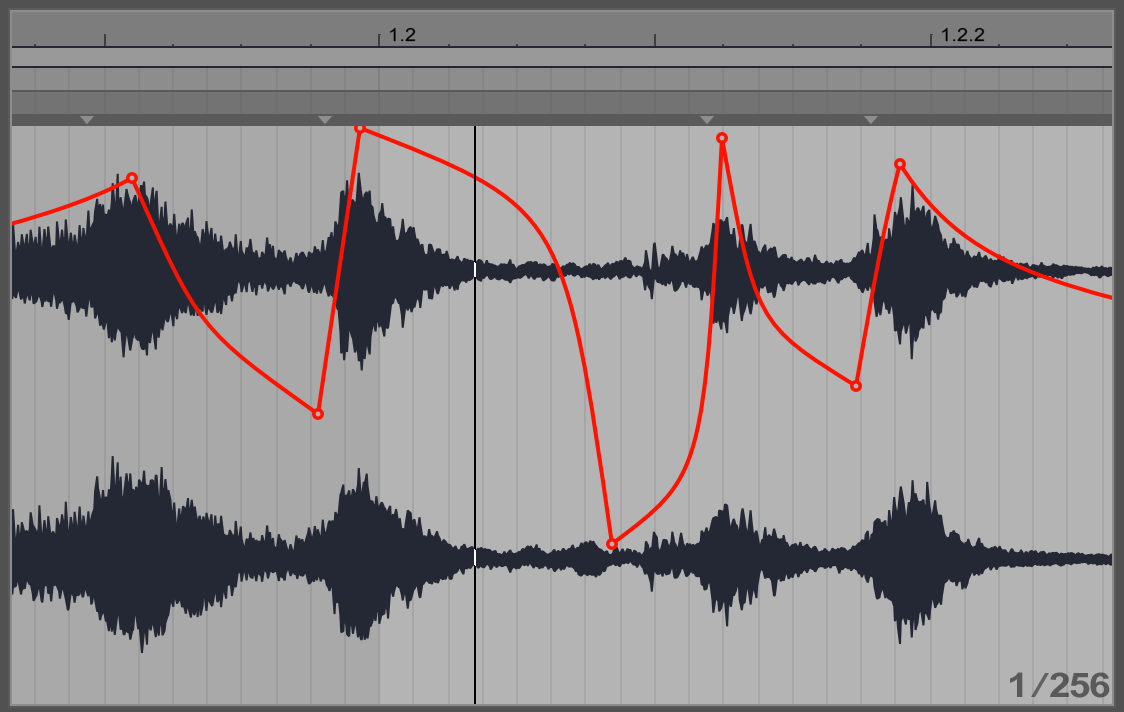
\includegraphics[width=\linewidth]{gfx/03_gesture/AbletonLiveAutomation_72dpi.png}
		\caption[Une courbe d'automation dans le logiciel Ableton Live]{Une courbe d'automation dans le logiciel Ableton Live, synchronisée à un échantillon audio.}
		\label{fig:gesture:automation}
	\end{minipage}
	\hspace{.02\linewidth}
	\begin{minipage}[t]{0.48\textwidth}
	  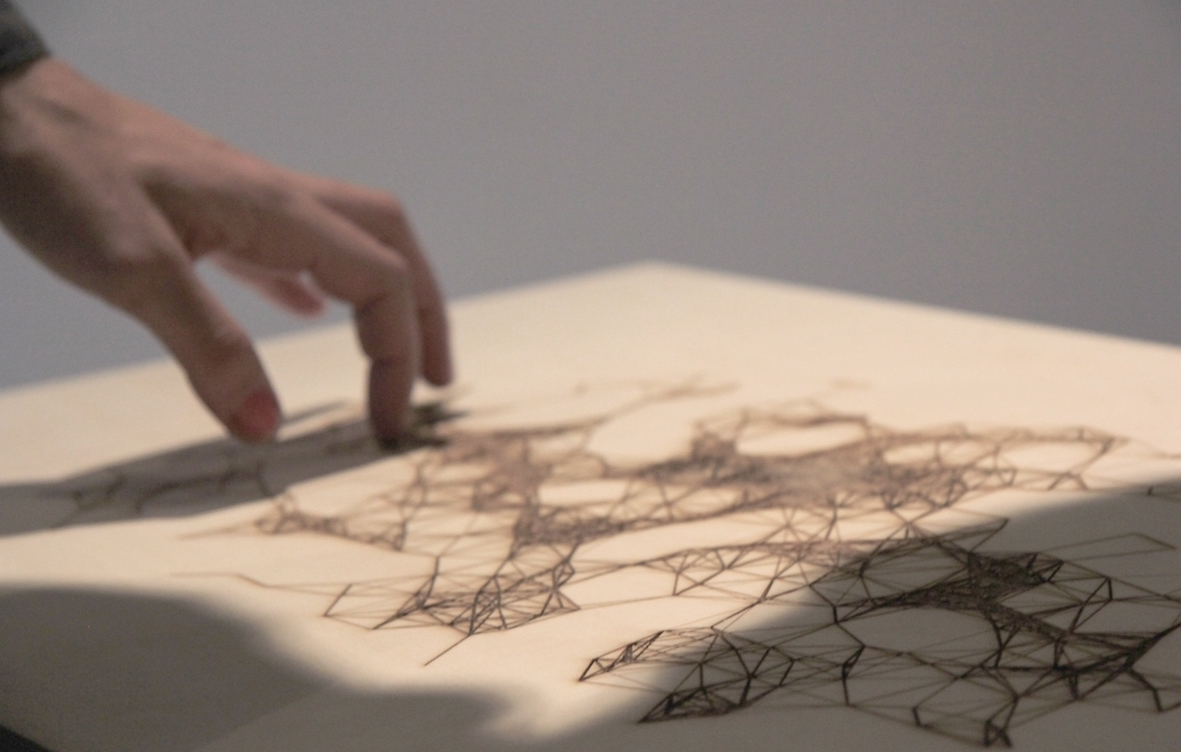
\includegraphics[width=\linewidth]{gfx/03_gesture/EnriqueThomas-TangibleScore.jpg}
		\caption[Partition tangible d'Enrique Tomás]{Partition tangible d'Enrique Tomás}
		\label{fig:gesture:tangible_score}
	\end{minipage}
\end{figure}
%------------------ Figure : geste programmé ---------------------
\\
\indent Stiegler développe le concept de ``gramme'' comme \iquote{corps organisé de signes et de symboles} et emprunte à Sylvain Auroux \cite{auroux_revolution_1994} le concept de ``grammatisation'' comme \iquote{le processus par lequel le continuum temporel des comportements humains est transformé en un spatial discret, qui permet de les intégrer dans les outils}. Ainsi en est-il de l'informatique, qui dissocie en symboles et en catégories discrètes ce qui est continu et intégré dans le geste, comme dans le son. Pour Stiegler, les objets sont des enregistrements\footnote{Stiegler utilise les termes de ``rétentions tertiaires'' pour décrire cette inscription de la mémoire dans les objets, afin de la mettre en perspective des ``rétentions primaires'' que sont la conscience du flux temporel et les ``rétentions secondaires'' que sont les souvenirs qui constituent l'expérience d'un individu.}, dans lesquels la mémoire de ce que nous faisons et de ce que nous connaissons est déposée sous la forme d'une mémoire technique.\\
\indent Le concept de Stiegler fait également écho à la notion de ``diagramme'', proposée par Gilles Deleuze dans son étude sur la peinture de Francis Bacon \cite{deleuze_francis_1981} : \iquote{Le diagramme, c'est donc l'ensemble opératoire des lignes et des zones, des traits et des taches asignifiants et non représentatifs. Et l'opération du diagramme, sa fonction, dit Bacon, c'est de suggérer. Ou, plus rigoureusement, c'est d'introduire des «~possibilités de fait~» : langage proche de celui de Wittgenstein. Les traits et les taches doivent d'autant plus rompre aevc la figuration qu'elles sont destinées à nous donner la Figure. C'est pourquoi elles ne suffisent pas elle-mêmes, elles doivent être «~utilisées~» : elles tracent des possibilités de fait, mais ne constituent pas encore un fait (le fait pictural).}\\
\indent On peut voir un parallèle frappant entre cette notion de diagramme et les fonctions assumées à la fois par l'instrument et par la partition musicale. L'instrument de musique contient ainsi l'enregistrement de la théorie musicale qui lui est propre (ses ``traits et ses taches'' que représentent son organisation des hauteurs, sa signature timbrale, son ergonomie, etc.) et que le luthier lui imprime. De même, on peut voir la partition comme un ``enregistrement'' de la pensée et du travail du compositeur, une trace de ses ``gestes sédimentés'' comme le dit Jean-Paul Olive dans \cite{olive_expression_2013}. La composition et la lutherie sont deux formes d’écriture diagrammatiques du geste et du son, qui s’inscrivaient jusqu’alors (avant le numérique) sur des médiums distincts: papier pour la composition, matériaux physiques pour la lutherie. Le numérique offre un médium commun qui permet leur recomposition mutuelle: l'instrument est ``composé'' \cite{schnell_introducing_2002}, la partition est ``instrumentalisée''\footnote{Voir à ce sujet le travail explicite de Enrique Tomás sur les ``partitions tangibles'' \cite{tomas_tangible_2014}} et les gestes de l'expression compositionnelle et de l'expression performative s'interpénètrent \cite{dobrian_e_2006}.\\
\indent Ces gestes programmés ne sont pas de simple enregistrements linéaire à repoduire tels quels, mais des modèles complexes et dynamiques\footnote{Cette idée est développée au chapitre \ref{sec:algorithms:MID}} qui invitent à l'interaction, au jeu\footnote{Cf. les propos de Stiegler dans \cite{stiegler_circuit_2004} \iquote{Quant à la duction de l'instrumentiste, elle vient retemporaliser ce qui ne peut être que spatial : le travail de la composition, ce n'est que spatial, c'est du temps spatialisé, et en cela, essentiellement en défaut d'être. C'est du virtuel pur. C'est du temps discrétisé et détemporalisé dans cette mesure. Discrétisé, il devient manipulable dans sa détemporalisation temporaire telle que la pratique le com­positeur, mais il n'est que virtuel. Il ne peut devenir actuel qu'avec l'interprète, qui doit le re-temporaliser.}}, par le musicien qui n'est pas, justement, un \textit{utilisateur} qui démarre, par exemple, la lecture d'un enregistrement audio. La performance musicale consiste justement à faire entendre ce qui n'est pas calculable comme le dit Stiegler \cite{stiegler_circuit_2004}: \iquote{Un musicien, c'est quelqu'un qui d'abord entend, c'est-à-dire qu'il est primordialement affecté par l'oreille, une oreille qui a cependant des yeux et des mains, et un corps qui les relie. Il ne se contente pas de calculer. Il peut calculer, il doit même calculer, mais s'il le fait, c'est pour donner à entendre ce qu'il a lui-même entendu comme l'incalculable même.}\\
\indent Ce jeu de la main et de l'oreille, qui vient mettre en mouvement ces \textit{gestes programmés} par un geste expressif incalculable, m'amènent à introduire l'idée de geste de ``re-sonnance'', qui se départit du modèle acoustique d'excitation/modulation, en ce qu'il nourrit une relation avec le son qui n'est pas simplement causale mais intègre l'idée d'agencement compositionnel et d'aller-retour entre la temporalité du geste re-sonnant et celle, intrinsèque au geste programmé.

%-------------------------------------------
\subsection{Le geste de re-sonnance}

\noindent Si les gestes programmés s'apparentent au résultat d'un processus de ``composition instrumentale''\footnote{Ce processus qui se décline sur différentes échelles temporelles est toutefois réalisables durant le temps même de la performance, en particulier dans le \textit{live-coding}.}, comment donc nommer ces gestes qui permettent de faire sonner un \gls{DMI} ? On ne peut se réduire à les nommer ``gestes d'excitation et de modulation'' (même si la métaphore qui les sous-tend peut s'appuyer sur cette idée), car de nombreux gestes n'évoquent en rien cette dimension physique (e.g. l'ouverture d'un fader de volume). On pourrait utiliser le terme de ``gestes effecteurs'' de Delalande, mais il faudrait les coupler d'une part à un processus dynamique, et d'autre part à une métaphore définissant leur logique. Or dans le cas de l'analyse du jeu pianistique de Gould, le piano est déjà sa propre métaphore, car l'instrument acoustique \textit{est} sa propre interface et son propre modèle intermédiaire à la fois\footnote{Ce qui n'empêche pas d'autres métaphores extra-pianistiques de se superposer à l'instrument et d'en orienter les gestes effecteurs, comme le note Delalande : \iquote{(...) les différents touchers sont pour lui [Gould, NdE] l'équivalent d'une orchestration pour différencier les parties polyphoniques; ainsi le staccato joue-t-il le rôle des \textit{pizzicati} de violon et le grand \textit{legato} de la basse, celui des violoncelles. Il n'est donc pas exclu que certains gestes puissent être dictés par cette imagination orchestrale (...)}}. La notion ``d'objet sonore-gestuel'' de Rolf Inge Godøy s'approche le mieux de l'idée présentée ici, en tant qu'elle intègre cette notion de métaphore intermédiaire entre le geste et le son, mais d'une part sa nature ``d'objet'' semble plutôt s'appliquer au modèle intermédiaire lui-même qu'au geste, et d'autre part Godøy semble (malheureusement) en limiter le cadre à une relation de congruence spectromorphologique entre le geste et le son (avec le dessein d'offrir, là-encore, une lisibilité de la relation énergétique).\\
%---- Figure : Guqin ---------
\begin{figure}[!t]
	\captionsetup{format=plain}%
	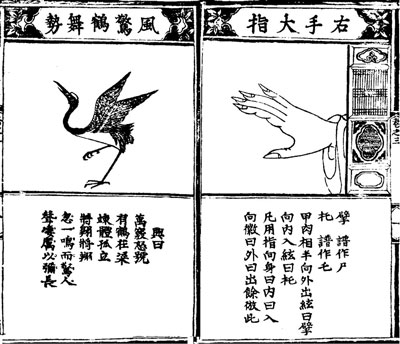
\includegraphics[width=\textwidth]{gfx/03_gesture/Guqin-hand01w.jpg}
	\caption[Le Tayin da quanji : métaphore poétique et animale dans la pédagogie du Guqin]{Un feuillet du \textit{Tayin da quanji} : les gestes instrumentaux du Guqin y sont décrits par un aphorisme poétique, et illustrés par le mouvement d'un animal. Source : cf. note \ref{fn:guqin}.}
	\label{fig:gesture:guqin}
\end{figure}
%---- Figure : Guqin ---------
\indent On pourra élargir ce cadre métaphorique au delà de la spectromorphologie en s'inspirant d'un système métaphorique un peu plus ancien et plus ouvert: le ``Tayin da quanji''\footnote{\label{fn:guqin}``L’Encyclopédie des sons suprêmes'', ouvrage ayant probablement vu le jour durant la dynastie Song, mais n'ayant survécu qu'à travers diverses éditions, une datant du \siecle{16}~siècle. Une reproduction est disponible en ligne : \url{http://www.silkqin.com/02qnpu/05tydq/ty3.htm}. Voir \cite{picard_chine:_1991}.} décrivant la relation gestuelle-sonore pour l'apprentissage du Guqin dans un ensemble de feuillets comprenant une illustration de la position de main, associée à l'image d'un animal et d'un texte poétique condensant l'esprit du mouvement (cf. figure \ref{fig:gesture:guqin}), par exemple : ``A la manière d'une grue qui danse parce qu'elle est effrayée par une brise.'' Considérons maintenant un hypothétique \gls{DMI} dont le modèle intermédiaire représenterait la danse de la grue durant la dynastie Song; le geste de re-sonnance d'un tel instrument pourrait consister à jouer la brise qui effraie la grue. Ce geste pourrait alors se concrétiser de différentes manières, que cela soit en simulant les mouvements du vent par le mouvement d'un stylet sur une tablette graphique, par le mouvement des mains munies d'accéléromètres, en soufflant dans un microphone, ou encore en pinçant des cordes sur lesquelles --~s'il est possible d'y évoquer la danse de la grue au Guqin~-- il serait sûrement possible d'évoquer le mouvement du vent.

\noindent J'utiliserai donc ici le terme de ``gestes de re-sonnance'' pour désigner un geste qui consiste à faire sonner un \gls{DMI} basé sur un ``geste programmé'', c'est-à-dire un modèle dynamique préalablement enregistré, encodé dans le \gls{DMI} et définissant son comportement. Son apparente similitude avec le terme \textit{résonance} n'est pas fortuite : le geste de re-sonnance a affaire à un processus qui possède sa propre dynamique avec lequel il doit s'accorder (ou non) et se mettre ``en résonance''.\\
\indent Le ``geste de re-sonnance'' s'appuie donc sur un \textit{modèle intermédiaire} projeté dans l'imaginaire par \textit{une métaphore} : modèle physique appelant des gestes d'excitation, modèle de lecture de vinyle appelant le \textit{scratching}, modèle de robinets-à-son\footnote{Je reprend ici l'expression utilisée par François Dumeaux pour décrire une partie de son interface de jeu. Cf. annexe \ref{appendix:dumeaux}.} controlés par l'ouverture de \textit{faders} sur une table de mixage, modèle cartographique (e.g. interpolation par boules) définissant un terrain à parcourir sur une tablette, modèle de grue effrayée dansant dans la brise, etc. Le geste de re-sonnance se déploie dans un espace polarisé par cette métaphore.\\
\indent Ce modèle est rendu tangible via l'interface, mais l'interface ne définit pas l'ensemble de la métaphore : ainsi un clavier peut servir au déclenchement de notes (comme sur sur un piano), mais si l'intensité des notes est contrôlé par un autre processus (e.g. une pédale d'expression, ou une foule d'agents virtuels autonomes) le clavier ne sera plus envisagé comme une surface ``de percussion'' mais comme un filtre, un crible ne laissant passer que certaines fréquences. Le métaphore du piano avec ses marteaux projetés par l'enfoncement des touches disparait pour laisser place à un autre rapport sensible à l'instrument.\\
\noindent \textbf{contextualité} A la différence du geste d'excitation/modulation/sélection de Cadoz à prétention universelle, le geste de re-sonnance est un geste \textit{contextuel}, dépendant de l'interface, du modèle intermédiaire, de la musique jouée, du contexte de performance. Cette contextualité n'empêche cependant pas qu'une typologie soit établie pour un contexte donné, en s'appuyant sur l'observation des pratiques qui s'y rattachent. C'est par exemple l'objet de la thèse de Baptiste Bacot \footnote{\cite{bacot_geste_2017}}: son analyse qu'il définit comme une \iquote{organologie située}, s'appuie sur l'observation de situations concrètes de performance musicale chez différents instrumentistes numériques, et prend en compte les spécificités de leur configurations instrumentales.\\
\indent C'est aussi le cas dans le travail mené par Nathanaëlle Raboisson et Pierre Couprie, sur l'étude du geste performatif dans l'interprétation de musiques acousmatique sur table de mixage \cite{raboisson_experience_2017}. Une analyse partant de l'observation méthodique des gestes et de leur corrélation (ou non) avec le résultat musical leur permet d'esquisser une typologie propre à cette pratique, incluant des \iquote{gestes de placement} qui participent à la (dé)construction de l'espace sonore, ou encore des \iquote{gestes d'accompagnement}\footnote{Le sens est ici tout autre que le geste d'accompagnement tel que défini par Delalande évoqué précédemment.} caractérisés par une synchronie entre le geste et la morphologie sonore.\\
\indent De même qu'il existe un répertoire gestuel associé aux instruments acoustique, les modèles intermédiaires définissent, de manière modulaire, un vocabulaire d'interaction qui leur est lié. Le geste de re-sonnance s'appuie donc sur les affordances et la structure musicale associées à certains modèles intermédiaires : un geste venant contrôler une boucle de batterie telle que le Amen Break peut s'appuyer sur l'ensemble des techniques de \textit{chopping}\footnote{Dans les musiques basées sur l'utilisation du break-beat, le chopping consiste à découper la boucle de certaines manière en segments plus petits afin de les reconfigurer dans un ordre différent.}, \textit{cutting}, \textit{filtrage} passe-bas, \textit{stuttering}, \textit{varispeed}, etc. qui lui sont historiquement associées.\\
\indent Norbert Schnell développe l'idée de ``ré-animation d'enregistrements audio''\footnote{Le terme anglais \textit{reenactment} utilisé dans son travail reflète mieux que ``ré-animation'' le lien avec la théorie de l'enaction sur laquelle s'appuie notamment son travail.} \cite{schnell_playing_2013} et propose une étude très riche sur le plan théorique comme sur le plan pratique des modalités d'engagement dans une relation gestuelle/sonore par le biais d'une action métaphorique. En particulier, plusieurs exemples s'appuient sur une pièce musicale complète (de Johann Sebastian Bach, en l'occurence) et présentent diverses stratégies possibles d'avancement dans la pièce, sur la base d'une même structure commune définie par l'œuvre de Bach.


\subsection{Résonance entre gestes re-sonnants et programmés}

\noindent Les instruments acoustiques présentent des modes de résonance que l'instrumentiste apprend à connaître, à apprivoiser, pour obtenir les qualités sonores qu'il ou elle recherche. Ces modes de résonance influent sur le timbre qui sera, par exemple sur un instrument à corde, rond et ample si l'on joue la corde au milieu de sa longueur, tandis qu'il sera plus grêle et chuintant si l'on joue \textit{sul ponticello}. La résonance de l'instrument acoustique peut également affecter d'autres paramètres que le timbre, par exemple le rythme : un percussioniste peut mettre à profit le rebond de ses baguettes sur la peau tendue, lors d'un jeu de roulements, et adaptera le poids et/ou la tension qu'il applique sur ses baguettes en fonction de la zone qu'il frappe et de son élasticité.\\
\indent Cette adaptation dynamique du geste à la résonance de l'instrument prend d'autres dimensions encore dans des \glspl{DMI}, pouvant générer de manière autonome toute une phrase musicale, tout un morceau. La nature dynamique et générative des \glspl{DMI} déplace l'agentivité\footnote{La notion d'agentivité dans la performance musicale dépasse sa simple implémentation opérante dans les \gls{IHM}. Par exemple, les figures dialogiques dans la musique classique ont été également analysée à travers ce prisme, voir notamment \cite{graybill_whose_2016}} de l'interaction instrumentale sur un terrain où elle se distribue entre des processus ``qui tournent'' et qu'il s'agit ``d'attraper''\footnote{Guerino Mazzola rapporte cette phrase du mathématicien Jean Cavaillès dans \cite{mazzola_topos_2018}: \iquote{Comprendre, c'est attraper le geste et pouvoir continuer}.} pour en jouer. Un exemple évident de cette situation est l'alignement rythmique entre deux morceaux mixés par un \gls{DJ}, ou encore l'utilisation d'un \textit{looper} permettant à un musicien de superposer plusieurs couches musicales et devant se jouer en rythme avec ce qu'il a enregistré.\\
\indent Le \gls{DMI} peut se retrouver en position de mener le jeu et imposer sa cadence à l'instrumentiste. La performance musicale avec un \gls{DMI} est donc une co-performance où la distribution du contrôle de la synthèse et de la gestuelle qui la provoque (ou en découle), peut se définir de manière polymorphe. Une partie de la dynamique de jeu peut être prise en charge par la machine et une autre partie par l'instrumentiste dans une relation qui peut parfois s'apparenter à un duo\footnote{Cette redistribution dialogique devient explicite dans des dispositifs tels qu'Omax (\cite{assayag_omax_2006}) ou le Continuator (\cite{pachet_continuator:_2003}). Voir par exemple la session d'improvisation entre György Kurtág père et fils avec le Continuator : \url{https://youtu.be/pqfKGlRvddg}.}.\\
\indent La part d'agentivité respective de la machine et du musicien dans la production du son des \glspl{DMI} définit en fait tout une échelle de nuances, allant de la posture de la personne écoutant la musique ``malgré elle'' (dans un supermarché, typiquement) à celle du musicien engageant tout son corps (physique et mental) dans l'interaction musicale. Cette recherche de la résonance avec l'instrument, qui vise à en comprendre l'organisation des sons et les rythmes propres, à en attraper les gestes programmés, à y trouver les \textit{sweet-spots} est peut-être, davantage que le medium constitutif de l'instrument, ce qui définit vraiment son instrumentalité. La possibilité des \glspl{DMI} de pouvoir générer du son en continu sans qu'aucun effort physique ne soit nécessaire pose en effet la question de l'engagement du musicien de manière plus critique encore qu'avec les instruments acoustiques car, à l'inverse, ne pas jouer peut requérir un effort physique.\\
\indent Les gestes du musicien peuvent alors entretenir diverses relations expressive ``en phase'' avec le mouvement autonome de l'instrument : dialogique, d'accompagnement, d'accentuation, ... mais il peut également s'affranchir d'une relation lisible au profit d'une subversivité expressive.

%%%%%%%%%%%%%%%% FIN de cette section ? %%%%%%%%

%%%%%%%%%%%%%%%%%%%%%%%%%%%%%%%%%%%%%%%%%%%%%%%%%%%%%%%%%%%%%%%%%%%%
%%%%%%%%%%%%%%%%%%%%%%%%%%%%%%%%%%%%%%%%%%%%%%%%%%%%%%%%%%%%%%%%%%%%


\section{Subversion sonore, subversion gestuelle}
\label{sec:gesture:subversion}
%------------------ Figure : geste lisible ou subversif ---------------------
\begin{figure}[!htbp]
	\captionsetup{format=plain}%
	\centering
	\begin{minipage}[t]{0.48\textwidth}
	  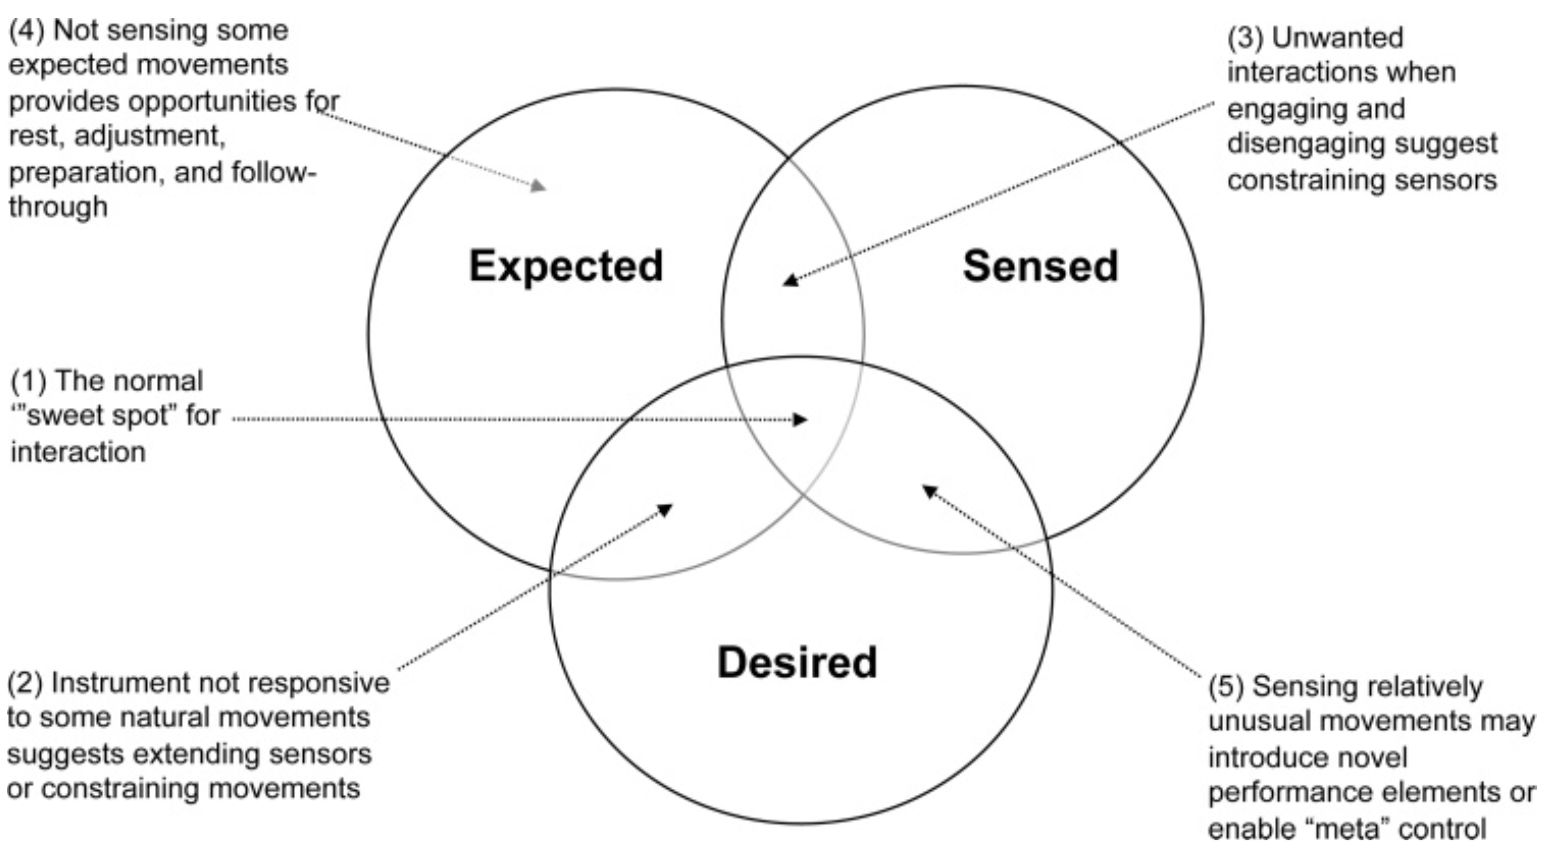
\includegraphics[width=\linewidth]{gfx/03_gesture/Benford_expected-sensed-desired.png}
		\caption[Gestes attendus, captés et désirés]{Gestes attendus, captés et désirés d'après \cite{benford_performing_2010}}
		\label{fig:Benford_expected-sensed-desired}
	\end{minipage}
	\hspace{.02\linewidth}
	\begin{minipage}[t]{0.48\textwidth}
		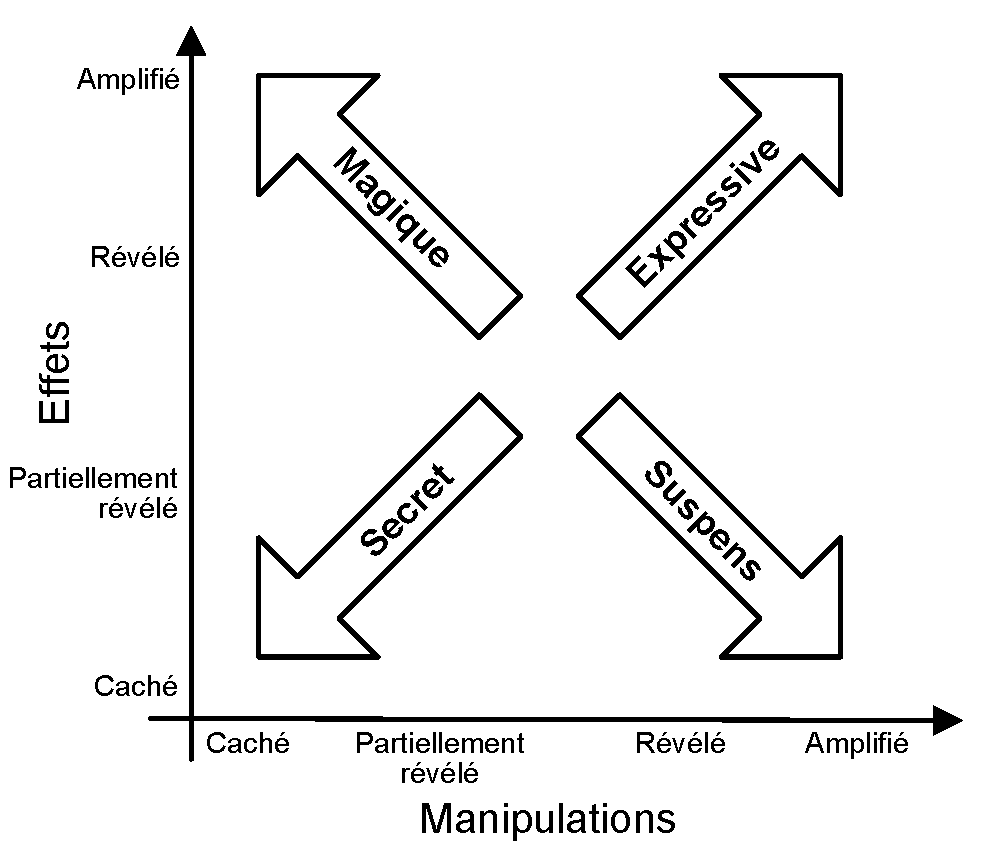
\includegraphics[width=\linewidth]{gfx/03_gesture/ManipulationVsEffect2.pdf}
		\caption[Stratégies de design d'interfaces pour le spectateur]{Stratégies de design d'interfaces pour le spectateur, d'après \cite{reeves_designing_2005, benford_performing_2010}}
		\label{fig:gesture:Benford}
	\end{minipage}
\end{figure}
%------------------ Figure : geste lisible ou subversif ---------------------
\subsection{Geste produit, capté, perçu}

\noindent Dans le domaine des \gls{IHM}, peu d'importance était accordée au geste en dehors de son interaction directe avec la machine jusqu'à la fin des années 1990, comme le dénote l'analyse de Gordon Kurtenbach dans l'ouvrage \textit{The art of human-computer interface design} : \iquote{Un geste est un mouvement du corps qui contient de l'information. Faire un signe d'au-revoir est un geste. Appuyer sur la touche d'un clavier n'est pas un geste car le mouvement d'un doigt dans sa course pour frapper une touche n'est ni observé ni signifiant. Tout ce qui importe est quelle touche est enfoncée.}\footnote{\iquote{A gesture is a motion of the body that contains information. Waving goodbye is a gesture. Pressing a key on a keyboard is not a gesture because the motion of a finger on its way to hitting a key is neither observed nor significant. All that matters is which key was pressed.} \cite{kurtenbach_gestures_1990}}.\\
\indent Pourtant, comme le rappelait à la même époque Richard Leppert, la nature intangible du son et de la musique est polarisée par l'expérience visuelle: \iquote{Précisément parce que le son musical est abstrait, intangible et immatériel (...) que l'expérience visuelle de sa production est cruciale, tant pour les musiciens que pour le public, pour situer et communiquer la place de la musique et du son musical dans la société et la culture. (...) La musique, malgré son immatérialité sonore phénoménologique, est une pratique incarnée, comme la danse et le théâtre.}\footnote{\iquote{Precisely because musical sound is abstract, intangible, and ethereal [...] the visual experience of its production is crucial to both musicians and audience alike for locating and communicating the place of music and musical sound within society and culture. [...] Music, despite its phenomenological sonoric ethereality, is an embodied practice, like dance and theater.} \cite{leppert_sight_1993}}

BOF : \textbf{Différence entre geste effectué et geste capté} : un son électroacoustique, par exemple une figure de ``delta'', pourra ainsi, avec un même geste de balaiement de la main, et une même interface de captation (e.g. un simple \textit{slider}), être engendré via un seuillage sur la valeur du \textit{slider} qui déclenche un échantillon, être produit de manière continue, en lisant l'échantillon comme si l'on déplaçait une tête de lecture, pourra avoir son intensité sonore fonction de la vitesse du geste ou pas, etc. On voit que pour un même geste, un même son, et un même capteur, les possibilités de relations entre le geste et le son sont multiples.

\noindent Nous avons vu dans les sections précédentes différents aspects concernant la fonctionnalité du geste, considérée du point de vue de l'instrumentiste. Ce point de vue privilégie généralement la recherche d'une relation lisible et cohérente entre le geste et le son, se situant à cette intersection où les actions permises par la configuration physique de l'agencement instrumental, celles effectivement captées par l'interface et celles désirées par l'instrumentiste se correspondent, ce que Steve Benford représente par le diagramme de Venn de la figure \ref{fig:Benford_expected-sensed-desired}. Ce diagramme fournit une représentation intéressante des compromis qui se présentent au luthier numérique pour la définition des gestes d'un \gls{DMI}. Benford remarque que si les zones où ces cercles ne se recoupent que partiellement peuvent apparaitre comme problématiques (interface pas assez sensible, gestes captés mais non-désirés), elles sont aussi des espaces permettant d'inventer de nouvelles relations (en particulier quand des gestes désirés qui peuvent être captés ne sont pas des gestes \textit{a priori} attendus).

\indent En se plaçant dans la perspective de l'instrumentiste, le diagramme précédent ne met pas en évidence la relation entre les gestes de l'instrumentiste et la traduction sonore de ces gestes par l'instrument, ni la perception de ce résultat par le spectateur-auditeur. Or, la compréhension du mapping entre gestes captés et production de l'instrument joue un rôle essentiel dans l'attribution de l'agentivité. En particulier, la représentation visuelle du fonctionnement de l'instrument peut aider à cette compréhension comme l'ont montré Florent Berthaut et al.\footnote{Cf. \cite{berthaut_rouages:_2013, berthaut_liveness_2015}.}. Benford propose un autre diagramme pour prendre en compte ces aspects que nous verront plus après, mais il nous faut d'abord éclaircir un point sujet à différentes orientations et partis-pris. 

\subsection{Une critique de la transparence}

\indent La poursuite exclusive d'une telle ``transparence instrumentale'', comme condition nécessaire à l'expressivité d'un instrument\footnote{Voir par exemple les remarques de Sydney Fels \cite{fels_mapping_2002} \iquote{We consider transparency as a predictor for expressivity. (...) We identify transparency as a quality of a mapping.}, Christopher Dobrian \cite{dobrian_e_2006} \iquote{Another basic need is that the software provide correspondences between input data and output sound that are sufficiently intuitive for both performer and audience.}, ou John Croft \cite{croft_theses_2007}}, pourrait masquer le fait que la relation entre le musicien et son public n'est pas exclusivement, sinon principalement, motivée par la recherche de cette transparence, comme l'ont notamment montré Canvan Fyans, Michael Gurevitch et Paul Stapleton dans une série d'articles\footnote{Cf. \cite{fyans_where_2009, fyans_examining_2010, gurevich_digital_2011}}. Il mettent notamment en évidence que la confiance apparente de l'instrumentiste joue un rôle prépondérant dans l'évaluation que fait le spectateur de la maitrise de l'instrumentiste et, de manière plus générale, que les modalités d'engagement des spectateurs dans l'appréciation et la compréhension d'une performance sont multiples et contextuelles.\\
\indent On pourra même arguer du contraire: que la subversion\footnote{Le terme ``subversion'' (du latin \textit{subvertere} : renverser, bouleverser) désigne \iquote{l'action visant à saper les valeurs et les institutions établies} (dictionnaire Larousse). Les moyens employés par la subversion consiste à diffuser un message contraire à un l'ordre établi, dans le but d'affaiblir celui-ci. Dans le cas de la musique, si la notion de subversion peut prendre une dimension culturelle ou politique dans certains courants musicaux, c'est ici au sens cognitif de la subversion de la perception que j'emploie ce terme. Par exemple, on pourra dire qu'un groupe de musique pop interprétant un tube en playback sur un plateau de télévision use d'un principe subversif, en laissant croire que ce que l'on écoute est le résultat de leur interprétation en direct (valeur établie), alors qu'il s'agit d'un enregistrement.} est une composante essentielle de la création artistique, qui se manifeste déjà le cas des instruments acoustiques. Leur design est en effet orienté par l'obtention d'une homogénéité de timbre tout à fait artificielle, autant que la discrétisation du \textit{continuum} des hauteur en notes. De même, les gestes du musicien et du compositeur crééent des continuités là où il y a discontinuité (e.g. le \textit{legato} sur des notes de piano, la modulation tonale pour passer d'un mode à un autre, la fusion des timbres dans le travail d'orchestre),  et inversement introduit des ruptures pour déjouer les attentes du public (e.g. les jeu de contre-temps rythmiques, le \textit{subito-piano}). La musique est un art du mirage, de l'illusion --~comme le rappelle Risset dans la citation en exergue de ce chapitre~--, dans lequel la transparence n'est qu'un alibi de la subversion, pour dessiner de nouvelles relations du sensible.\\
\indent L'attribution de qualités expressives aux \glspl{DMI} sur la base de la perception explicite de causalité entre ce que fait le musicien et le son produit, traduit ainsi une référence implicite à un modèle instrumental acoustique qui n'est qu'à moitié justifiée. Loin de prétendre ici que le modèle causal de l'instrument acoustique soit obsolète, il semble nécessaire de s'en détacher si l'on veut saisir l'étendue réelle des possibilités créatives offertes par les \glspl{DMI}. L'expressivité ne saurait être réduite à la simple traduction sonore immédiate des gesticulations d'un musicien. Les films de la nouvelle vague, en particulier le cinéma de Jean-Luc Godard ou Wim Wenders, ont suffisamment prouvé que la collision de plans sonores et visuels n'entretenant \textit{a priori} aucun rapport de causalité ou de synchronicité, sont capable de susciter une émotion intense et de capturer un fragment inouï ayant pu se glisser dans la fêlure des normes\footnote{Et que rappelle ce refrain de Leonard Cohen dans \textit{Anthem}: \iquote{Ring the bells that still can ring / Forget your perfect offering / There is a crack, a crack in everything / That's how the light gets in}.}, comme le fait le poème qui s'affranchit de la grammaire habituelle pour inventer la sienne propre.\\
\indent Les \glspl{DMI} offrent de nouvelles possibilités de subversion de la perception --~comme autant de fêlures du modèle acoustique~-- qui peuvent s'appuyer sur les caractéristiques qui leur sont propres. Ainsi, le découplage énergétique permet des correspondance inattendues entre force du geste et intensité du son, les capacités d'enregistrement permettent de faire surgir des matériaux de toute nature sonore, l'absence potentielle de contact avec l'instrument permet d'associer plus librement gestes effecteurs et gestes d'accompagnement, et la reconfiguration dynamique des algorithmes permet d'envisager une métamorphose continue des relations de jeu.\\

\subsection{Stratégies expressives d'interaction gestuelle}
%------------------ Figure : geste lisible ou subversif ---------------------
\begin{figure}[!htbp]
	\captionsetup{format=plain}%
	\centering
	\begin{minipage}[t]{0.48\textwidth}
		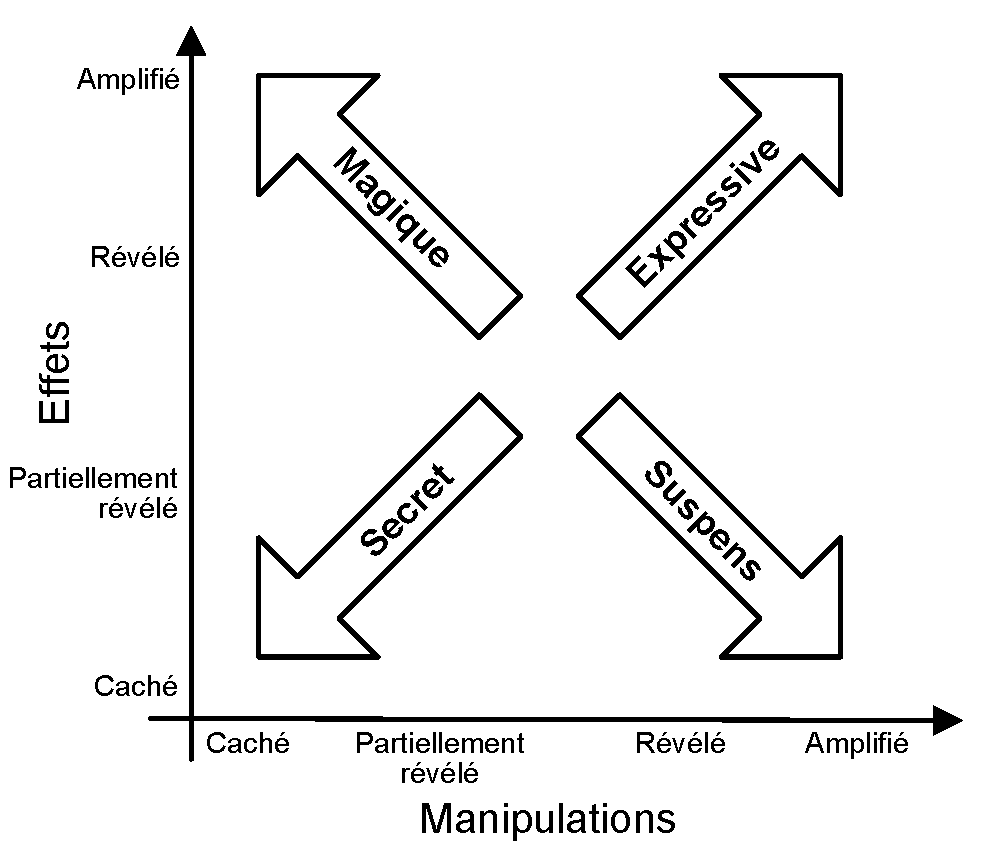
\includegraphics[width=\linewidth]{gfx/03_gesture/ManipulationVsEffect2.pdf}
		\caption[Stratégies de design d'interfaces pour le spectateur (schéma de Benford)]{Stratégies de design d'interfaces pour le spectateur, d'après \cite{reeves_designing_2005, benford_performing_2010}}
		\label{fig:gesture:Benford}
	\end{minipage}
	\hspace{.02\linewidth}
	\begin{minipage}[t]{0.48\textwidth}
		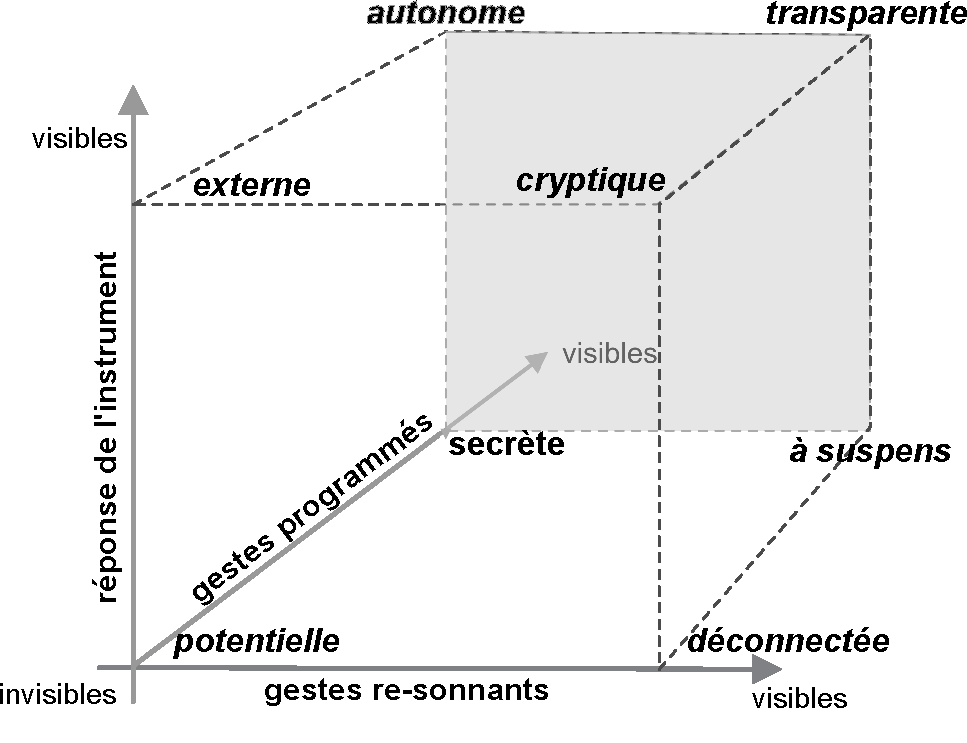
\includegraphics[width=\linewidth]{gfx/03_gesture/SubversiveCube.pdf}
		\caption[Stratégies de design d'interfaces pour le spectateur (schéma proposé)]{Stratégies de design d'interfaces pour le spectateur}
		\label{fig:gesture:expressive-spaceold}
	\end{minipage}
\end{figure}
%------------------ Figure : geste lisible ou subversif ---------------------

\begin{figure}[!htbp]
	\captionsetup{format=plain}%
	\centering
	\begin{minipage}[t]{0.8\textwidth}
		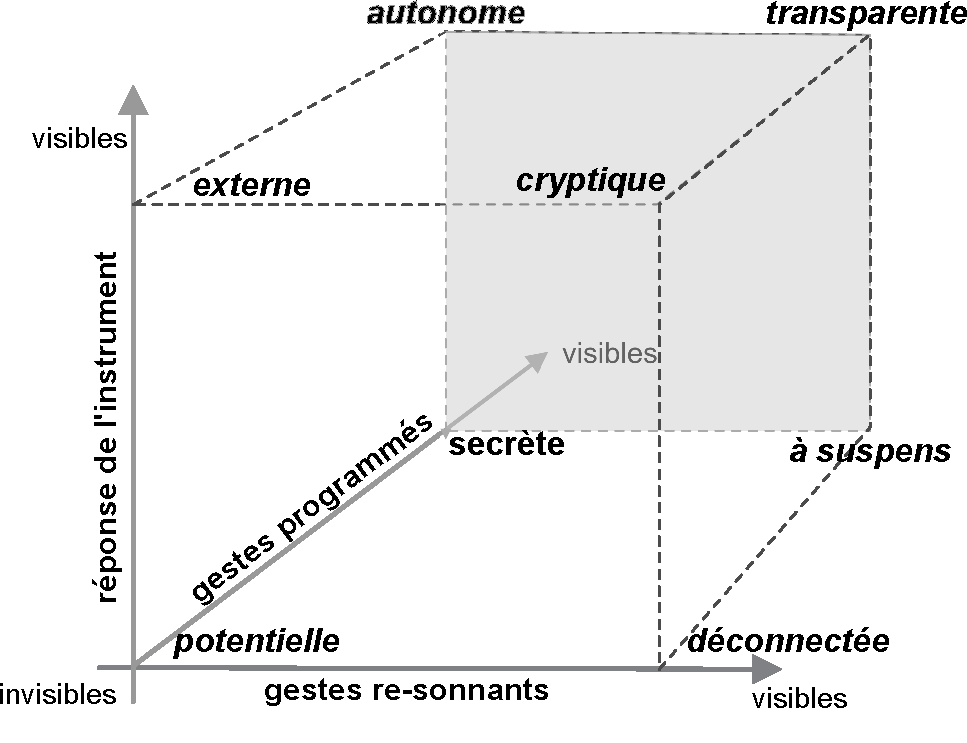
\includegraphics[width=\linewidth]{gfx/03_gesture/SubversiveCube.pdf}
		\caption[Stratégies de design d'interaction instrumentale pour le spectateur]{Stratégies de design d'interaction instrumentale pour le spectateur}
		\label{fig:gesture:expressive-space}
	\end{minipage}
\end{figure}
%---------------

\noindent Dans une analyse des stratégies de design d'interface en fonction de leur perception par le spectateur \cite{reeves_designing_2005}, Stuart Reeves, Steve Benford et al. distinguent quatre orientations possibles en fonction du degré de visibilité des gestes effecteurs de l'instrumentiste par rapport au degré de perceptibilité (visible, audible) de l'effet produit par l'instrument (cf. figure \ref{fig:gesture:Benford}):
\vspace{-1em}
\begin{itemize}[noitemsep]
 	\item \textbf{expressive} lorsque les gestes de manipulation et les effets sont perceptibles, l'interface est dite \textit{expressive}; 
 	\item \textbf{occulte}: à l'opposé, une interface sur laquelle les gestes effecteurs sont invisbles ainsi que le résultat est jugée ``occulte'' (\textit{secretive}) — Benford évoque le cas d'une performance qui ne serait accessible qu'à une partie du public. Ce pourrait être aussi le cas par exemple lors de gestes discrets visant à rappeler des réglages sur l'instrument et dont l'effet n'est pas directement perceptible; 
 	\item \textbf{à suspens}: si des gestes effecteurs sont visibles manifestement destinés à produire un effet mais qu'aucun effet n'est perçu, cela pourrait être perçu comme un dysfonctionnement, mais également (et c'est l'orientation proposée ici par Benford) comme un moment de \textit{suspens}, si le public a conscience que l'action de ces gestes lui seront perceptibles plus tard. Benford prend l'exemple d'un public faisant la queue devant une installation dont il ne peuvent faire l'expérience que lorsque leur tour arrive. On pourrait aussi observer une telle situation dans des gestes de live-coding, où le code s'écrit de manière visible pour le public\footnote{Une pratique courante dans le live-coding consiste à montrer son écran au public, généralement sous la forme d'une vidéoprojection du code composé en direct (cf. manifeste TOPLAP : \url{https://toplap.org/wiki/ManifestoDraft})}, dont l'activation est imminente, mais dont on ne perçoit le résultat qu'une fois le code envoyé dans le \gls{DSP};
 	\item \textbf{magique}: enfin, et c'est la direction qui m'intéresse plus particulièrement ici, les gestes effecteurs peuvent être cachés tandis qu'un effet est produit par l'instrument, configuration que les auteurs appellent ``magique''.
\end{itemize}
%-----------------
\noindent Ce schéma présente l'intérêt de dépasser une vision uni-dimensionnelle de l'expressivité instrumentale, envisagée comme le seul résultat du degré d'agentivité de l'instrumentiste perceptible par l'auditeur/spectateur, en proposant une caractérisation de la relation geste/son prenant en compte l'absence potentielle (et potentiellement souhaitée) de congruence entre les gestes effecteurs de l'instrumentiste et leur traduction sonore perçue par le public.\\
\indent On pourrait cependant ajouter une dimension à ce schéma en y insérant le paramètre de cohérence de la relation entre les gestes effecteurs et l'effet produit\footnote{Le schéma de Benford semble se placer dans le cas particulier où cette relation \textit{est} cohérente.}. Cette cohérence peut être définie comme la congruence énergetico/spatio/temporelle du geste et du son\footnote{Telle que préconisée par Cadoz\footnote{Cf. supra p. \pageref{sec:gesture:ergotic}.}, ou John Croft dans \cite{croft_theses_2007}}, mais de manière plus générale, elle se caractérise par la capacité des spectateurs-auditeurs à comprendre cette relation, qu'elle soit congruente ou non\footnote{Ce qui semble être démontré par l'étude de Berthaut et al. dans \cite{berthaut_rouages:_2013}}. Pour conserver les mêmes unités d'axe, je propose d'assimiler ce paramètre de \textit{cohérence} au degré de ``visibilité des gestes programmés'', qu'il faut ici entendre comme une compréhension de la mécanique interne de l'instrument, de son mapping. On obtient ainsi un espace tri-dimensionnel dans lequel d'autres axes d'interprétation de la relation expressive se dessinent (cf. figure \ref{fig:gesture:expressive-space}).\\
\noindent Ainsi, le schéma que je propose ici se fonde sur celui de Benford, en reformulant certains de ses axes et en l'étendant selon l'axe de la visibilité du \textit{geste programmé} :
\vspace{-1em}
\begin{itemize}[noitemsep]
	\item \textbf{transparente} : il me semble ici préférable de renommer la zone désignée comme \iquote{expressive} dans le schéma de Benford par le terme \iquote{transparent}, afin de s'affranchir de cet abus de language qui empêche de considérer d'autres formes d'expressivité que celle passant par la transparence de la relation instrumentale.:
	\item \textbf{autonome} : de même, la zone désignée comme \iquote{magique} me semble davantage correspondre à une situation d'\iquote{autonomie} de l'instrument. En particulier, la notion de geste magique\footnote{Le geste magique a notamment été analysée par Marcel Mauss dans \cite{mauss_esquisse_1902}, et plus spécifiquement dans le cadre des \gls{IHM} dans \cite{lokuge_dynamic_1995, marshall_deception_2010}} implique d'autres variables que celles de l'occultation et de la révélation, en particulier l'inscription dans une temporalité permettant de créer un contexte favorable à la subversion (par la narration, le détourement d'attention, etc.). La notion d'autonomie se traduit par exemple dans le rôle pris par une platine vinyle jouant un enregistrement en l'absence de geste venant perturber sa lecture;
	\item \textbf{cryptique} : une relation sera vue comme cryptique si les gestes re-sonnants et le résultat sonore ne présente aucune relation apparente;
	\item \textbf{externe} : dans le cas où un effet sonore est perceptible mais qu'aucune action ne semble les produire, ni celles de l'instrumentiste, ni celles provoquées de manière autonome par l'instrument, le son sera perçu comme externe à l'instrument. Cette situation est typiquement renforcée dans le cas des instruments électroniques par la distance fréquente entre l'instrument et les haut-parleurs qui supprime cette congruence de localisation entre l'instrument et le son, naturelle dans les instruments acoustiques. La présence fréquente d'un espace scénique mis en lumière focalise bien évidemment l'attention sur l'instrument[iste], mais ce point de fuite de l'attention peut être précisément être déplacé par ces même procédés (e.g. être situé hors de la scène);
	\item \textbf{déconnectée} : un musicien procédant à des mouvements sur un instrument dont le public ne peut pas voir le fonctionner (ou le supposer) renvoie l'impression d'un instrument déconnecté et mutique. Cette sitation se rencontre par exemple lorsqu'un musicien numérique procède à réglages en amont de sa performance ou entre deux morceaux musicaux ou lorsque, effectivement, l'instrument ne répond pas;
	\item \textbf{potentielle} : enfin la seule présence de l'instrument, sans qu'aucun geste ne lui soit adressé, sans qu'elle ne produise aucun son, ni que son fonctionnement ne soit compréhensible pourrait s'apparenter à ce qui se passe lorsque nous faisons la \textit{rencontre} d'un instrument inconnu, ou d'un objet dont nous envisageons l'instrumentalité. Que nous portions intentionnellement notre attention sur cet objet, où que notre attention soit guidée sur elle (e.g. par sa mise en lumière dans un espace dédié tel qu'une scène ou une gallerie d'art), il subsiste le mouvement de notre imagination qui projette les affordances, le jeu, les sonorités potentielles. La pièce \textit{4'33"} de John Cage ou encore l'installation ``Handphone table'' de Laurie Anderson (cf. figure \ref{fig:gesture:HandphoneTable}) se situent à la limite de ce cas de figure.
\end{itemize}

%------------------ Figure : geste lisible ou subversif ---------------------
\begin{figure}[!htbp]
	\captionsetup{format=plain}%
	\centering
	\begin{minipage}[t]{0.8\textwidth}
		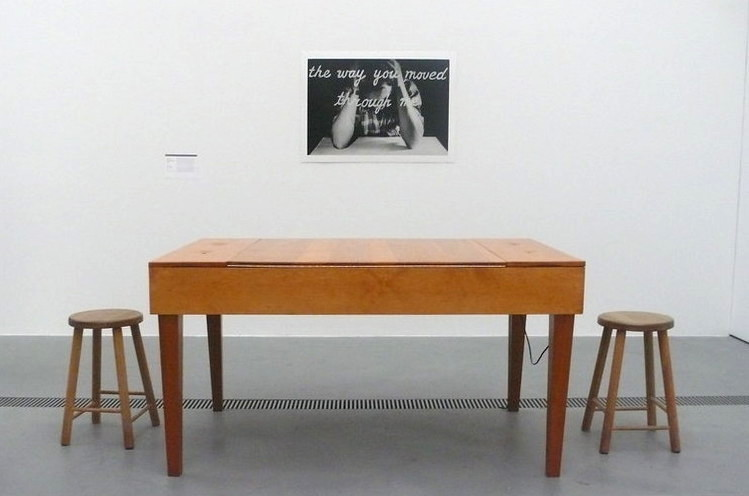
\includegraphics[width=\linewidth]{gfx/03_gesture/LaurieAnderson-HandphoneTable-PhotoLuisaRibas.jpg}
		\caption[\textit{Handphone table} de Laurie Anderson]{\textit{Handphone table} de Laurie Anderson. Photographie:Luisa Ribas}
		\label{fig:gesture:HandphoneTable}
	\end{minipage}
\end{figure}
%---------------

\indent Il faudrait rajouter à ce schéma une variable permettant de définir si le comportement de l'instrument est désiré ou subi, en particulier lorsque la relation n'a pas cette ``transparence'' généralement considérée comme celle attendue de la part d'un instrument. En présentant ces différents rôles comme des stratégies plutôt que seulement des problèmes, nous prenons ici le parti de les considérer comme des fonctionnement souhaités par le musicien. Dans la mesure où ils seraient subis, on pourra les assimiler à la notion de fausse note, dont le musicien peut tout à fait s'accomoder en les réutilisant dans la dynamique du jeu, selon le désormais célèbre adage répété par de nombreux jazzmen dont Miles Davis qu'il n'y a pas de ``fausses notes'' en tant que telles, que ce sont les notes jouées ensuite qui les rendent justes ou fausses\footnote{Herbie Hancock en rend compte dans une interview, en notant le caractère ``magique'' de la résolution trouvée par Miles Davis : \iquote{I played this chord that was so wrong. I thought I had destroyed everything(...) Miles took a breath and he played some notes, and he made my chord right. I could not figure out how he did that, that sounded like magic.} cf. \url{https://youtu.be/C-GrRIgdmW8}}.\\
\indent L'assertion de Mile Davis (et d'autres) sur le caractère de ``justesse'' d'une note\footnote{Le terme de justesse est ici utilisé au sens de sa pertinence, son intérêt, et non pas de la précision de hauteur par rapport à un système tonal.} dépendant de ce qui est joué à sa suite fait apparaître deux autres lacunes importantes de ce schéma : sa dimension temporelle d'une part et la connaissance préalable des idiomes musicaux et instrumentaux sur lesquels se construit à la fois la performance et la construction de sens de la part du spectateur. Ainsi, on ne peut subvertir la perception de l'auditeur qu'à la condition qu'il y ait un système de valeur à déconstruire. Ce système peut exister préalablement à la performance (e.g. ``un piano produit un son de piano''), mais aussi se construire durant le temps même de la performance, en installant une relation qui semble cohérente et stable, au point de sembler établie.\\
\noindent Analysons ici les différents cas de figures amenant à la perception d'une relation subversive pour le spectateur. 
 
%-------------------------------------------
\subsection{Sons paradoxaux, gestes paradoxaux}

De la même manière que l'écriture musicale sur papier a permis de développer des processus de compositions difficilement pensables sans ce support visuel \footnote{tels que la rétrogradation ou la fugue}, les ordinateurs ont permi de créer des formes sonores qu'il aurait été impossible de concevoir sans cet outil computationnel, tels que les sons paradoxaux de Risset et Shepard \footnote{Ce qui ne signifie pas que les sons paradoxaux soient impossible à produire sans recourir à l'ordinateur; cf. leur interprétation vocale par Victoria Hart \url{https://vimeo.com/147403169}}.

%---- Figure : gesteReelGesteSuppose ---------
\begin{figure}[!htbp]
	\captionsetup{format=plain}%
	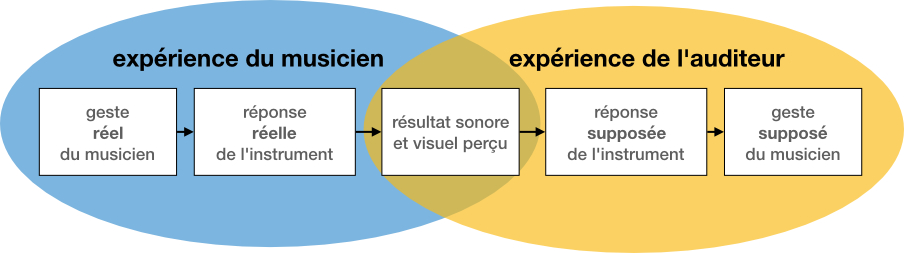
\includegraphics[width=\textwidth]{gfx/03_gesture/gesteReelGesteSuppose.jpg}
	\caption{Geste produit, geste perçu, fonctionnement réel et supposé de l'instrument}
	\label{fig:gesture:RealVsSupposed}
\end{figure}
%---- Figure : gesteReelGesteSuppose ---------


\subsubsection{Gestes feints}

\noindent Tout d'abord, se présente le cas où les gestes ne sont pas cachés, mais où subsiste un décalage entre les gestes perçus par le public et les gestes effectivement captés par l'instrument. Ce cas de figure peut se présenter sur des instruments acoustiques (et \textit{a fortiori} sur des \glspl{DMI} expressifs). Par exemple, dans certaines pièces pour piano de György Kurtág, le pianiste doit effectuer un geste d'approche énergique vers le piano, laissant supposer qu'il va jouer \textit{forte}, mais le retenir au dernier moment pour jouer \textit{pianissimo}\footnote{Ce mode de jeu a été observé en concert dans une interprétation des \textit{Játékok} de Kurtág. Après vérification, l'indication n'est pas explicite dans la partition, mais fait partie des instructions données par György Kurtág en vue de l'interprétation de certaines parties, d'après son fils György Kurtág Jr. On y trouve par contre l'indication inverse, consistant à jouer \textit{fortissimo} \iquote{en touchant les touches sans faire de son}}. L'oreille se prépare à entendre un son intense et s'en protège par un réflexe stapédien\footnote{Le réflexe stapédien est la contraction involontaire des deux muscles de l'oreille moyenne, le muscle stapédien et le muscle du marteau. En rendant plus rigide la chaîne des osselets, il atténue le niveau des sons transmis à l'oreille interne.}, renforçant ainsi l'intensité du \textit{pianissimo}.\\
\indent Au delà de cet exemple particulier, il existe de nombreux moyens pour l'instrumentiste de ``tromper'' l'auditeur/spectateur pour lui faire entendre ce qu'on veut lui faire entendre, plutôt que ce qui est vraiment présent en terme acoustique. Des doigtés alternatifs sur les vents sacrifiant la justesse pour obtenir la fluidité d'enchainement, au gestes accompagnateurs qui en étendent la perception dans l'imaginaire\footnote{Nattiez, Music and discourse p44 : certain pianistes ont l'impression de donner de la ``profondeur'' à un accord en permettant aux doigts de glisser vers l'intérieur du piano après avoir enfoncé les touches. (...) inversement, Braendel : le son de notes soutenues sur le piano peut être modifié... à l'aide de certains mouvements qui rendent la \textit{conception du cantabile} du pianiste visible pour le public. (Delalande, ``vers une psycho-musicologie'' in L'enfant du sonore au musical):166, (Brendel, A. 1976. Musical Thoughts and Afterthoughts. Princeton: Princeton University Press. p.31)}, 

\subsubsection{Gestes du playback}

\noindent Nous avons également utilisé des gestes feints dans la performance \textit{FIB\_R} réalisée avec Gladys Brégeon, pour jouer une partie dont la ryhmique très précise et machinique. La rigueur métronomique requise n'étant atteignable qu'en la confiant à l'ordinateur, nous effectuons des gestes en rythme avec cette séquence autonome, ce qui laisse au spectateur l'impression que nous la jouons nous-même et contribue au l'esthétique générale de cette performance dans laquelle le rôle occupé par la machine et par les performeurs demeure ambigüe.

\subsubsection{Capteurs dissimulés}

\noindent Les auteurs mentionnent deux exemples utilisant des contrôleurs invisibles pour le public (des pédales de type \textit{foot-switch} supposées peu visibles d'une part, et l'utilisation de capteurs dissimulés dans le corps d'un instrument traditionnel, dont l'action est masquée par les gestes habituels du musicien.)

\subsubsection{Mapping non-conventionnel}

\noindent Dans ce cas de figure, les gestes ne sont pas cachés à proprement parler, mais le résultat de leur action défie certaines règles faisant partie de l'expérience du spectateur, par exemple si l'on fait correspondre un son très doux à un geste violent et inversement.

\iquote{Dans le domaine du geste, les outils technologiques peuvent bien sûr jouer un rôle complice, démultipliant les perspectives, inversant les conséquences attendues, décelant l'infime ou captant par méthode statistique tel ou tel paramètre du jeu musical.} 
\iquote{(...) s’approprier à la manière d’un mime les gestualités sonores qui, malgré les indications de la partition, ne peuvent être réellement considérées et donc interprétées que via le prisme de l’écoute.}
P. Jodlowsky \cite{jodlowski_geste_2006}

\subsubsection{Métamorphisme du mapping}

\noindent Il n'est pas nécessaire de se baser sur des lois ancrées dans l'expérience collective, mais également possible de déjouer des règles qui ont été établies en cours de jeu, en modifiant dynamiquement le fonctionnement de l'instrument pendant le jeu. Il devient nécessaire dans ce cas de faire en sorte que la ``couture'' entre les différents réglages qui se succèdent soit invisible, soit en procédant par un changement continu (e.g. interpolation vers de nouveaux réglages), soit en transposant dans le nouvel espace de jeu un certain nombre de paramètre de l'ancien espace de jeu afin qu'ils correspondent\footnote{Un exemple concret est donné dans la vidéo présentant les Modèles Intermédiaires Dynamiques (cf. chapitre \ref{ch:algorithms}) : la transition entre les différents modèles présentés se fait en conservant une cohérence visuelle de la représentation (e.g. la position, l'orientation des formes) --~ alors que tout le comportement à changé \url{https://vimeo.com/25740547} .)}.

\indent Cependant, le jeu de l'instrumentiste est polarisé par le fait qu'il joue (généralement) pour un public. La réception de la performance par le spectacteur/auditeur engage une projection active de sa part pour reconstruire du sens : déterminer la cause des sons, anticiper les trajectoires, ...  Cette projection se construit sur la base de l'expérience du spectateur et constitue l'objet central de la recherche en psychologie de la perception.


Celle-ci est prise dans une perception globale impliquant le geste du musicien, la réaction de l'instrument ainsi que les projection active de causalité de la part du spectateur sur la scène à laquelle il assiste.

L'étude de la perception des \glspl{DMI} est arrivée plus tardivement que l'étude de leur contrôle mais a pris une importance croissante ces vingts dernières années, notamment à cause de la considération dans le domaine des \textit{IHM} de scénarios narratifs dans ce que l'on nomme ``l'expérience utilisateur''. 

(Auslander, Croft, Bin, Fyans, Benford)


Au delà du timbre et des modes de jeu que le luthier ``programme'' dans l'élaboration d'un instrument acoustique, les \glspl{DMI} permettent d'élaborer une programmation qui à la particularité de pouvoir se déployer dans le temps avec une certaine autonomie, d'y dessiner un trajet\footnote{On peut mettre en regard la notion de trajet, qui suit un chemin, avec celle de plan   \iquote{la notion de référence s'est développée avec la masse grandissante des faits enregistrés, mais les écrits sont chacun une suite compacte, rythmée par des sigles et des notes marginales, dans laquelle le lecteur s'oriente à la manière du chasseur primitif, le long d'un trajet plutôt que sur un plan.} dans \cite{leroi-gourhan_geste_1964}, p 69}, voire d'y construire une narration. 

\iquote{Les propos des instruments qui nous entourent ne sont pas obligatoirement les nôtres. Ils appartiennent à ceux qui ont fait produire les instruments. Les détourner, c’est se libérer. Les instruments récents sont fascinants parce que, plus que tout autre, ils abritent des virtualités ignorées et parce qu’ils permettent des actions libératrices.} Villem Flusser, in ``les gestes''


Les métaphores définissant les relations gestuelles-sonores peuvent être guidées par la recherche d'une certaine lisibilité, comme il a été le cas dans la plupart des travaux pré-cités, qu'elle soit de nature énergétique, spectromorphologique, ou imitative d'instruments existants. Ces relations peuvent toutefois être envisagées dans leur aspect subversif, en profitant de la perception différenciée de l'instrumentiste et de l'auditeur/spectateur.

Un exemple significatif est l'interprétation de ``Hangsimogato N°2'' de György Kurtág Jr\footnote{Vidéo disponible sur \url{https://www.youtube.com/watch?v=MJ8Z5skovLw}}. Dans cette pièce, le développement musical se fait par avancement sur une partition pré-programmé par l'intermédiaire d'un capteur Infra-Rouge (D-Beam). Le capteur lui-même n'est pas sensible à l'orientation de la main ou à quelle main (gauche ou droite) vient couper le rayon, mais György Kurtág Jr développe un vocabulaire gestuel qui établit des relations de correspondance avec les différents son de la pièce. Ces relations de correspondance peuvent s'appuyer sur une similarité de morphologie énergétique, mais dans certains cas (e.g. geste de présentation des mains ouvertes vers le ciel, replis des bras en croix) elle sont purement métaphoriques et poétiques.
\todo{rajouter un screenshot de la vidéo de Gyorgy}



Toutes les composantes du son, de la musique, et de la scénographie sont sujettes à l'invention de gestes, selon ce que le musicien décidera comme d'importance pour sa musique.



Perception d'erreur du point de vue du spectateur \cite{fyans_ecological_2012}

\cite{emerson_gesture-sound_2018}

Reeves et Benford propose un modèle de stratégies pour le design ``d'interfaces spectateurs'' montrant les effets obtenus lorsque la manipulation (les gestes de l'instrumentiste dans le cas qui nous intéresse ici) et l'effet de cette manipulation (le son dans notre cas) présentent chacun des degrés divers de visibilité.

Dans la figure de Benford manque la possibilité que la visibilité ne soit pas causale de l'effet.
Ce qui nous manque ici est la possibilité que la partie visible de la manipulation ne sont pas la cause de l'effet.

La cohérence\footnote{J'appelle ici ``cohérence'' la causalité \textbf{apparente} entre le geste et le son, pour la distinguer de la causalité \textbf{effective}, avec laquelle elle est mise en regard. La littérature en psychologie cognitive utilise cependant davantage le terme de perception de causalité.} entre le geste et le son se base sur un ensemble de valeurs qui ont été analysée dans de nombreux articles de sciences cognitive\footnote{Voir par exemple \cite{michotte_perception_2017} qui compile un grand nombre d'effets amenant à une perception congruente}, en particulier celles de la théorie de la perception, telles que :
\vspace{-1em}
\begin{itemize}[noitemsep]
	\item la congruence temporelle : syncrhonisme, destin commun, si j'entend le son en même temps que le geste, alors c'est ce geste qui a produit ce son.
	\item la congruence spatiale : si j'entend le son venir d'un endroit précis et que l'instrument se trouve à ce même endroit, alors le son vient de l'instrument.
- médiation par un objet intermédiaire dont on pense connaître le fonctionnement
\end{itemize}


\vspace{-1em}
\begin{itemize}[noitemsep]
	\item \textbf{lisible} : la perception du geste et du son apparait cohérente par rapport au système. Par exemple : on voit et on entend une personne parler.
	\item \textbf{illisible} : on voit une personne parler et on entend une autre voix
	\item \textbf{troublante} : c'est le cas du ventriloque : il est bien responsable du son que l'on entend (causalité), mais l'absence de mouvements de lèvre rend la perception visuelle incohérente avec la parception sonore (dissonance cognitive entre vue et ouïe).
	\item \textbf{subversive} : c'est le cas du playback
\end{itemize}

\subsection{Définition} 


La subversion peut intervenir à différents niveaux. Au niveau de la composition, l'écriture musicale permet des modulations qui déjouent les attentes de l'auditeur. (e.g. Pink Floyd, breathe transition). Elle peut également se situer au niveau du jeu, en usant de procédés comme des gestes qui contredisent ce qu'on entend et vont l'amplifier. Gyorgy Kurtag Jr. geste violent pour jouer une nuance pianissimo.

Exemples comparés de Applebaum Aphasia et Vincent Carinola/Jean Geoffroy "Virtual Rhizome".
BBC Classic Album: "Pink Floyd - The Dark Side of the Moon"

Dissonance cognitive.

Synchrèse de Michel Chion.

Parler du playback, du air-guitar, de la synchrèse.



Bien que ces catégorisations du gestes décrivent adéquatement différents aspects du geste instrumental sur des instruments acoustiques, il semble que le geste musical intègre une aspect subversif souvent négligé.

En particulier, dans le cas des \glspl{DMI}, la relation entre le geste et le son est totalement sujette au design de ce que l'on nomme communément le \gls{mapping} et la part de subversion devient partie intégrante du design de ce mapping. 


Il semble dès lors que l'on peut envisager d'autres types de relation entre le geste et le son, afin de tenter de décrire les différents rapports qu'ils entretiennent selon les situations.

Risset fait remarquer l'importance de l'histoire du son d'origine mécanique dans la perception des sons \cite{risset_son_1992}: \iquote{II semble à première vue que l'acoustique numérique puisse s'affranchir de la mécanique. Cependant notre ouïe a évolué dans un environnements d'objets vibrants: aussi la prise en considération des contraintes et des particularités des vibrations mécaniques est-elle importante pour comprendre les idiosyncrasies de la perception auditive et pour en tirer parti.
Les limites de l'acoustique numérique dépendent des capacités différentielles de perception davantage que des contraintes mécaniques. Pourtant, notre perception auditive est orientée par un monde de sons produits mécaniquement, et la mécanique ne doit pas être écartée de façon cavalière, comme l'ont suggéré les travaux de Gibson et Cadoz : les spécificités des vibrations mécaniques mettent en lumière l'organisation perceptuelle dans le processus auditif. \footnote{The limitations of digital acoustics depend upon the differential capacities of perception rather than upon the constraints of mechanics. Yet our auditory perception is geared to a world of mechanically-produced sounds, and mechanics should not be given a cavalier dismissal, as the work of Gibson and Cadoz has suggested : the specifics of mechanical vibrations shed light on the the perceptual organization in the hearing process.} TODO : traduire l'anglais, plus riche.}

\vspace{-1em}
\begin{itemize}[noitemsep]
\item Gestes emphatique = en phase avec le mouvement interne du son
\item Geste apophatiques = en opposition de phase avec le son
\item Geste unrelated
\end{itemize}




Risset, Kurtag Jr., Kurtag Père


aspect scénographique de la performance musicale.
\vspace{-1em}
\begin{itemize}[noitemsep]
\item \textbf{gestes de feintes} : (rupture) déception de l'attente, mais visible après coup. E.g. dans le football, faire semblant d'aller à droite et envoyer le ballon à gauche, en musique: ommettre le temps fort d'un rythme bien établi, etc. La mécanique du geste est entièrement visible mais a été confuse par un changement innatendu.
\item \textbf{geste magique} : La mécanique du geste reste invisible et la logique causale entre le geste et son résultat reste inexplicable, et sujette à spéculation imaginaires.
\end{itemize}


%---- Figure : Triggering modes ---------
\begin{figure}[!htbp]
	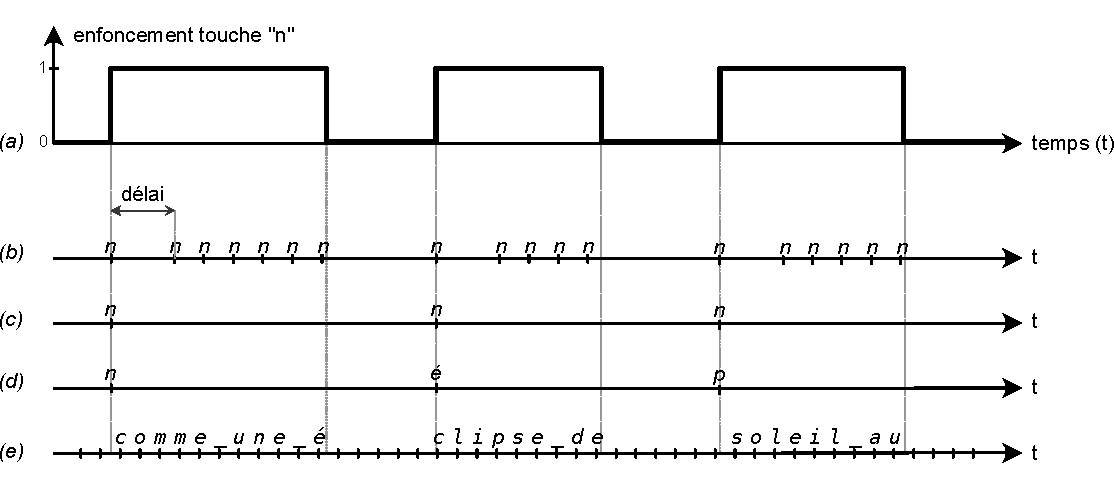
\includegraphics[width=\textwidth]{gfx/03_gesture/key_modes.pdf}
	\caption{Différents modes de déclenchement: (a) enfoncement de la touche ``n''; (b) comportement habituel d'un clavier (e.g. dans un traitement de texte) (c) suppression de la répétition (d) utilisation d'un réservoir (e) phrases séquencées rythmiquement}
	\label{fig:gesture:triggering_modes}
\end{figure}

%%%%%%%%%%%%%%%%%%%%%%%%%%%%%%%%%%%%%%%%% 
\section{Conclusion}
\label{sec:gesture:conclusion}


\noindent On voit donc que la relation entre le geste et l'instrument a été considérablement affectée par l'introduction de l'électricité, mais plus encore du numérique, dans le corps de l'instrument. Ces relations se construisent sur un medium présentant des caractéristiques radicalement opposées à celles de l'instrument acoustique : l'absence de causalité et de continuum énergétique entre le geste et le son, le métamorphisme du comportement de l'instrument, et l'absence possible de contact physique entre le geste et l'instrument.

Dans ce contexte, plusieurs voies sont possibles. 
La recherche d'une lisibilité de la relation geste/son peut s'appuyer sur des modèles physiques recréant artificiellement les conditions perdues de l'instrument acoustique, ou encore sur des relations basées sur la relation spectro-morphologiques entre mouvements du geste et mouvements du son.

Ces gestes peuvent également s'appuyer sur une connaissance du déroulement interne d'un matériaux enregistré, auquel cas une relation de re-sonnance / résonance vient définir une modalité de relation instrumentale ou les mouvements gestuels ne sont pas nécessairement dans une relation mimétique, mais viennent s'articuler sur différents plans de jeu mêlant écoute, extrapolation imaginaire, [ré]agencements à la volée et anticipatifs, gestes muets dont l'action n'est perçue que de manière différée, etc.


De même que l'on peut travailler une partition et devenir expert dans son interprétation, on peut travailler un instrument pour en devenir expert et travailler les différentes compositions pour cet instrument. On peut aujourd'hui travailler le geste (et l'écoute!) et en devenir expert pour jouer les différents instruments qui s'offrent à ces gestes.


La possibilité de modéliser dans les \glspl{DMI} non seulement la traduction du geste en son (mapping), mais également la représentation de son influence (visualisation du mapping), ou encore les aspects métaphoriques auquel on l'associe (prodiction de son et d'image musicales) nécessite de prendre en compte la totalité de ses aspects phénoménologiques, sémiotiques, poétiques pour le design des \glspl{DMI}. 
\indent La synthèse des différentes approches ayant contribué jusque la à cette compréhension, ainsi que les propositions de nouvelles catégories et de nuances par rapport à ces modèles contribue, je l'espère, à l'avancement de sa compréhension dans cette perspective.


Il est important de comprendre qu'il n'y a plus de relation fixe entre le geste. La relation se définit de manière contextuelle et fait partie d'un lutherie généralisée qui englobe à la fois des aspects compositionnels et des aspects de lutherie plus traditionnelle.


=> Comment ces aspects influencent le design de l’instrument ?
De cette étude du geste instrumental, on peut retenir plusieurs éléments qui viennent orienter (todo, better word) le développement des briques de bases qui constituent les \glspl{DMI}.

\vspace{-1em}
\begin{itemize}[noitemsep]
\item transgression des catégories (entre continu et discret, entre audio et non-audio, création de relation arbitraires entre paramètres orthogonaux)
\item absence de limites arbitraires dans les représentations numériques (e.g. ambitus de pitch, polyphonie maximale)
\end{itemize}

\vspace{-1em}
\begin{itemize}[noitemsep]
\item \textbf{le format de données} : doit permettre le polymorphisme (cf. Zicarelli ``numbers without meaning'') entre les diverses formes de captation du geste (signal, événement, présence stable ou éphémère, etc.)
\item \textbf{le mapping} entre variables est lui-même sujet à une reprogrammation dynamique durant le jeu
\item \textbf{les différents gestes} de composition, de performance, d'écoute font partie intégrante des gestes de lutherie
\end{itemize}




\iquote{Si ça se trouve, cette notion que dans quelques années, ``tout sera possible avec la technologie'' fera que cela sera compliqué de créer un mystère entier et profond, parce que les gens du coup diront ``oui, j'en ai entendu parler, maintenant on peut faire ça''.
 J'ai un ami (...) qui a fait voler un espèce de morceau de tulle au dessus des gens avec des principes mécaniques, et beaucoup de gens disaient ``ah oui, c'était incroyable mais je pense que c'était un drône'', alors que pas du tout. Mais je me suis dit, c'est vrai que d'ici quelques années, un objet qui vole tout seul en silence dans l'espace, n'aura plus le même pouvoir de mystère qu'il y a quelques années.} Yann Frish dans \url{https://www.youtube.com/watch?v=5BqHXbQC36M}




\section*{extra material}
Notion de vivadi

Part of the excitment in the domain of new digital musical instruments in the 21st century can be attributed to the fact this fact as the musical creativity goes beyond the sound itself and includes the system through which it is performed. A downside of this situation, however, is that the novelty and digital features if the instruments create a sense of discontinuity with tradition , alienation, and lack of understanding by the audience as to what the instrument or the performer is actually doing.
\cite{magnusson_sonic_2019}



\iquote{Si ça se trouve, cette notion que dans quelques années, ``tout sera possible avec la technologie'' fera que cela sera compliqué de créer un mystère entier et profond, parce que les gens du coup diront ``oui, j'en ai entendu parler, maintenant on peut faire ça''.
 J'ai un ami (...) qui a fait voler un espèce de morceau de tulle au dessus des gens avec des principes mécaniques, et beaucoup de gens disaient ``ah oui, c'était incroyable mais je pense que c'était un drône'', alors que pas du tout. Mais je me suis dit, c'est vrai que d'ici quelques années, un objet qui vole tout seul en silence dans l'espace, n'aura plus le même pouvoir de mystère qu'il y a quelques années.} Yann Frish dans \url{https://www.youtube.com/watch?v=5BqHXbQC36M}





Subversion du geste : Kagel et le théâtre musical.
\url{https://geste.hypotheses.org/gemme}

\iquote{Dans le domaine du geste, les outils technologiques peuvent bien sûr jouer un rôle complice, démultipliant les perspectives, inversant les conséquences attendues, décelant l'infime ou captant par méthode statistique tel ou tel paramètre du jeu musical.} 
\iquote{(...) s’approprier à la manière d’un mime les gestualités sonores qui, malgré les indications de la partition, ne peuvent être réellement considérées et donc interprétées que via le prisme de l’écoute.}
P. Jodlowsky \cite{jodlowski_geste_2006}



\noindent Jakobson (1960) :
\vspace{-1em}
\begin{itemize}[noitemsep]
\item \textbf{expressive function}
\item \textbf{representational function}
\item \textbf{conative function}
\item \textbf{phatic function}
\item \textbf{metalingual function}
\item \textbf{poetic function}
\end{itemize}

\noindent David McNeil : 
\vspace{-1em}
\begin{itemize}[noitemsep]
\item \textbf{Iconics} where the gesture resembles the referent (e.g. describing an action or shape of an object with the hands).
\item \textbf{Metaphorics} where the vehicle (the gesture) relates in one of a number of metaphorical ways to the tenor (non-literal meaning) of the gesture, e.g. indicating a container or conduit for ideas, or a gift of an idea or suggestion (cf. Lakoff et Johnson 1980).
\item \textbf{Beats} where the hand, head, eybrows move roughly in synchrony with the rhythm of often emphatic speech, mark a sequence, or a hiatus such as a change of theme or focus.
\item \textbf{Cohesives} which create a gestalt in gesture space which is coextensive with a spoken utterance or – hierarchically – with its parts.
\item \textbf{Deictics} which may indicate an actual physical position, size, distance or direction, but may also place concepts metaphorically in physical gesture space
\end{itemize}


La mémoire et les gestes:
Leroi Gourhan

\iquote{Quant à l’action relayée (force motrice et transmission), elle domestique pour les utiliser des éléments qui étendent et complètent les effets techniques. Dans ce stade évolué, on n’est plus dans le faire mais dans le faire faire, engagé dans la voie techno-scientifique qui ne garde du geste humain initial que ses épures et en analyse indéfiniment les schèmes.} Michel Guérin, \cite{guerin_philosophie_2018}




Partant de l'idée que le geste et la musique sont deux phénomène impliquant le mouvement, je chercherai donc à définir l'intention gestuelle en fonction du rapport qu'il entretient avec le mouvement musical.
On peut dès lors envisager trois attitudes principales :
\vspace{-1em}
\begin{itemize}[noitemsep]
\item \textbf{jouer avec} : en phase avec le mouvement de la musique (geste emphatique), en soutenant par un rythme ou une harmonie complémentaire à ce qui est joué
\item \textbf{jouer contre} : jouer contre le mouvement pour chercher à l'annuler ou le détruire (geste apophatique)
\item \textbf{jouer indifféremment} : sans chercher à être ni contre, ni avec
\end{itemize}

On pourra nuancer cette catégorisation brutale en ajoutant une quatrième catégorie, qui se situerait entre 
le jeu ``avec'' et le jeu ``contre'' qui consiste à jouer en ``interférence'', c'est-à-dire qui vient infléchir une direction


\iquote{J'appelle technique un acte traditionnel efficace (et vous voyez qu'en ceci il n'est pas différent de l'acte magique, religieux, symbolique). Il faut qu'il soit traditionnel et efficace. Il n'y a pas de technique et pas de transmission, s'il n'y a pas de tradition.} Marcel Mausse, les techniques du corps

Il manque un élément important dans cette considération de la tradition. Pour qu'une tradition soit transmise, il faut que des individus la transmette. Cela peut se faire par la contrainte ou un système doctrinal (e.g. un système religieux), mais en cette absence de coercition physique ou mentale, la tradition sera transmise à la condition que les individus croient en la valeur de cette tradition et qu'ils lui accordent suffisament d'importance pour en mémoriser les principes.


%-------------------------- Figure : Shannon ----------------------------------
\begin{figure}[!htbp]
	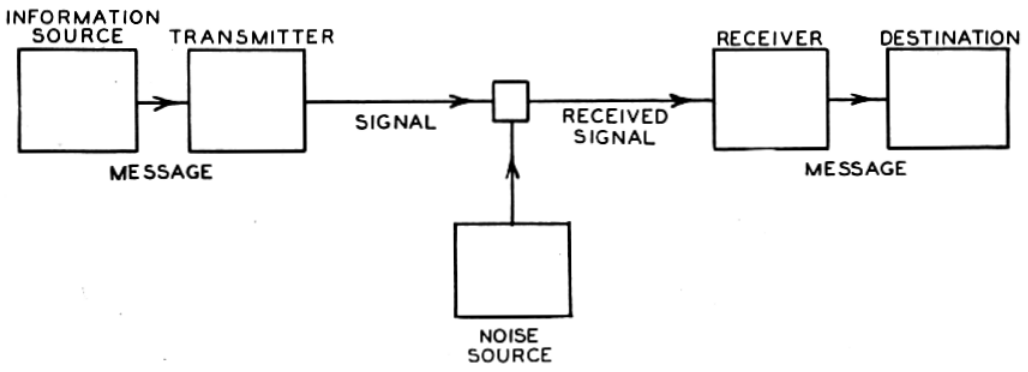
\includegraphics[width=\textwidth]{gfx/03_gesture/ShannonCommunicationSystem.png}
	\caption{Diagramme schématique d'un système général de communication, tel que proposé par Shannon.}
	\label{fig:gesture:shannon}
\end{figure}



Ces deux catégories de geste d'action et de gestes perçu sont emprunt de la théorie de l'information proposée par Shannon \cite{shannon_mathematical_1948} qui envisage la communication comme un système émetteur-message-récepteur unidirectionnel. 
L'inconvenient d'envisager le geste comme simple émetteur d'un signal (qu'il soit travail ou signe) est qu'il empêche de considérer le geste dans la rétroaction dans laquelle il s'inscrit avec l'instrument. En particulier dans la performance musicale, la rétroaction multimodale (par l'ouïe, la vue, le toucher) entre les geste d'un instrumentiste et son instrument, le son et le public est essentielle.

Il était tentant de l'appliquer à la situation musicale et de voir dans le phénomène sonore un message circulant du musicien vers l'auditeur, et les analyses du geste instrumental s'appuyant sur cette solide base théorique ont permis de développer un certain nombre de concept encore utile pour l'analyse du geste musical.

Cependant, la situation de performance musicale est loin d'être aussi fonctionnelle que celle qui consiste à vouloir transmettre un flux de données. Notamment, la théorie de l'information s'applique à des machines qui ignore totalement le contenu sémantique de ces données et les aspects cognitifs ou les références culturelles des émetteurs et récepteurs.
%-------------------------- Figure : transparence Fels -----------------------
\begin{wrapfigure}[14]{R}{0.5\textwidth}
	\begin{center}
 		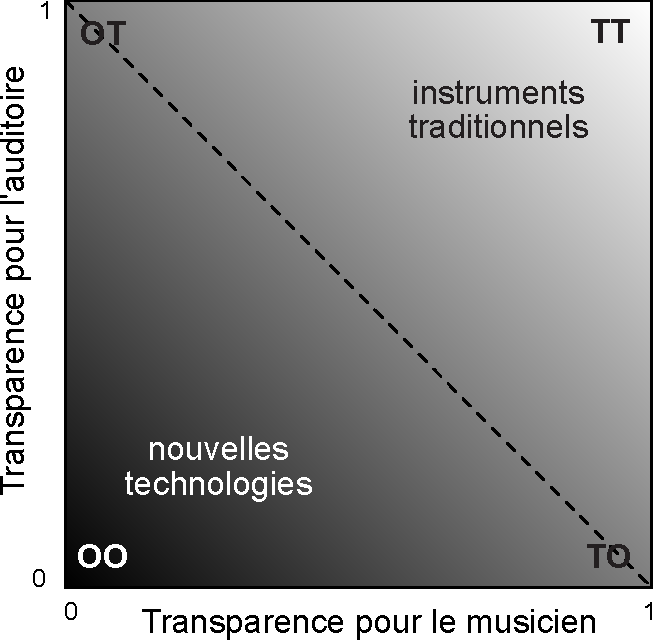
\includegraphics[width=0.48\textwidth]{gfx/03_gesture/Fels-transparency.pdf}
	\end{center}
	\caption{Transparence pour le musicien et l'auditoire, d'après \cite{fels_mapping_2002}}
	\label{fig:gesture:fels_transparency}
\end{wrapfigure}
%-------------------------- Figure : transparence Fels -----------------------

Certains auteurs ont critiqué cette approche \cite{fyans_where_2009} en remarquant que l'idée selon laquelle une connaissance et une compréhension préalable de l'instrument et de l'idiome était nécessaire pour évaluer une performance musicale, ne pouvait être généralisée aux \glspl{DMI}, à cause de l'émergence rapide de technologies, d'instruments et de pratiques de performance dans ce domaine. 

Cependant, cette critique reste ancrée sur une approche qui considère que le spectateur évalue le \textit{succès} d'une performance selon sa compréhension des intentions de l'instrumentiste.


Le jeu musical joue en partie sur l’attente de l’audience (récompensée ou non) sur la base de règles d'harmonies, d’idiomes (e.g. cadences, résolutions, cycles rythmiques), de citations (e.g. via le sampling), etc..
Affordance des instruments ne peut être réduite aux objectifs d’affordance des IHM.


Kurtag Jr. Hangsimotato (video)
Jean Haury Meta-Piano
Applebaum Aphasia

gestes incongruent (Musical gestures, Godoy, p.48)


Charlotte Moorman and Name June Paik performing John Cage’s 26’1.1499” for a String Player (Human Cello section

%%%%%%%%%%%%%%%%%%%%%%%%%%%%


Si le geste est un mouvement accompagné d'intention, il faut prendre en compte cette partie intentionelle et essayer de la qualifier, dans la perspective des conséquences qu'elle porte au design des \glspl{DMI}.

La notion ``d'image de son (i-son)'' de François Bayle exprime la mécanique psycho-poétique de construction de l'œuvre musicale acousmatique. Sa nomenclature ne se prête pas facilement à une application directe dans la lutherie (numérique ou non).
En partant de la classification des fonctions de l'écoute proposée par Pierre Schaeffer et Michel Chion (\cite{chion_guide_1994}, p.26) (Insérer ici le tableau comprendre-écouter-entendre-ouïr), François Bayle retient notamment trois niveaux d'écoute attentive (en regroupant entendre et comprendre dans un seul niveau) qu'il fait correspondre à trois niveau d'intentionalité dans la mise en jeu des \textit{images-de-sons}:
\vspace{-1em}
\begin{itemize}[noitemsep]
\item \textbf{\textit{im-son}}: l'image isomorphe, iconique, référentielle;
\item \textbf{\textit{di-son}}: le diagramme, sélection de contours simplifiés, indiciels ;
\item \textbf{\textit{mé-son}}: la métaphore ou métaforme, reliée à une généralité
\end{itemize}

Ces trois catégories font également écho au catégories de Delalande (gestes effecteurs, gestes accompagnateurs, gestes figurés) — sans qu'il y ait toutefois de relations causales triviales entre ces catégories du gestes et de l'écoute.

%------------------ Bricout: g-son -------------------------
Concept de \textit{g-son} proposé par Bricout \cite{bricout_les_2011}, à partir du concept d'i-son (\textit{image-son}) proposé par Bayle, comme ``dépassement de la suggestion de l'image par le son lui ajoutant de manière beaucoup plus évidente la suggestion du geste, de l'élan physique.''

Romain Bricout : couple ``déclenchement/modulation'' (analogue à l'archétype ``percussion/voix'' Martin Laliberté) comme atomes gestuels constitutif de tout mouvement. => NON tout l'espace gestuel avec toutes les connotations possibles (sémiotiques, mimétiques)

Bricout :
\iquote{Déclenchement et modulation représentent donc ces deux gestes primordiaux, à la base de de n'importe quel autre geste plus complexe. Par voie de conséquence, n'importe quel son renvoie lui-même à un geste producteur qui se rapprochera tantôt du déclenchement, tantôt de la modulation ou, par combinaison, des deux à la fois}
=> qu'en est il d'un field recording ?
%------------------ END Bricout: g-son -------------------------

J'aurais plutôt tendance à employer le terme ``d'image de geste'' (i-geste) pour décrire cette analogie entre les plans d'interprétation du geste et du son.

Le travail de création des correspondances entre geste et son passe ainsi par trois étapes faisant écho à ces différents niveaux de perception/compréhension musicale :
\vspace{-1em}
\begin{itemize}[noitemsep]
\item \textbf{coder} la relation algorithmique (causale ou non), c'est-à-dire concrètement la relation algorthmique qui s'opère entre les signaux captés par l'interface et le contrôle de la synthèse sonore, 
\item\textbf{jouer} la relation sensible, c'est-à-dire pratiquer (chorégraphier) l'ensemble du mouvement gestuel dont une partie seulement sera captée par l'interface de jeu;
\item\textbf{imaginer} la relation poétique, cette relation s'établit sur un ensemble plus complexe de valeurs esthétiques, de références culturelles impliquant de manière plus globale les questions de composition, de scénographie, de métaphores portée par les sons, etc.
\end{itemize}




\subsubsection{Les unités sémiotiques temporelles}

La définition des UST est donnée dans \cite{timsit-berthier_les_2004}:
\iquote{Les UST sont des segments musicaux, qui possèdent une signification temporelle en raison de leur organisation morphologique et cinétique. Elles peuvent êtres considérés comme des représentations iconiques qui entretiennent des rapports de ressemblance avec des modèles temporels naturels. L’UST ne traduit pas le phénomène musical à son niveau acoustique, mais cherche à y trouver en quelque sorte une intentionnalité.}



%%%%%%%%%%%%%%%%%%%%%%%%%%%%%%%%%%%%%%%%%%%%%%%%%%%%%%%%%%%%
%%%%%%%%%%%%%%%%%%%%%%%%%%%%%%%%%%%%%%%%%%%%%%%%%%%%%%%%%%%%
%%%%%%%%%%%%%%%%%%%%%%%%%%%%%%%%%%%%%%%%%%%%%%%%%%%%%%%%%%%%
%%%%%%%%%%%%%%%%%%%%%%%%%%%%%%%%%%%%%%%%%%%%%%%%%%%%%%%%%%%%
%%%%%%%%%%%%%%%%%%%%%%%%%%%%%%%%%%%%%%%%%%%%%%%%%%%%%%%%%%%%
%%%%%%%%%%%%%%%%%%%%%%%%%%%%%%%%%%%%%%%%%%%%%%%%%%%%%%%%%%%%
%%%%%%%%%%%%%%%%%%%%%%%%%%%%%%%%%%
\section*{Espace du geste musical}
La musique a longtemps été considéré comme étant faite d'un sous-ensemble de sons, les sons harmonieux, voire harmonique, avant qu'au \siecle{20}~siècle, les bruits n'y fassent leur place avec les avant-gardes, futuristes. 

John Cage in \cite{cage_silence:_1961}
\begin{quotation}
\noindent If this word, music, is sacred and reserved for eighteenth- and nineteenth-century instruments, we can substitute a more meaningful term: organization of sound.\\
\end{quotation}


Anecdote De Laubier ` le haut parleur ne fonctionne pas'

La musique n'est donc pas faite que de sons, au sens acoustique du terme, mais également (avant tout?) de la perception des sons, qui implique des processus de cognition, des références socio-culturelles, et une sensibilité, une mémoire propre à chacun. 
Ainsi, l'espace de la musique ne se présente non pas comme un sous-ensemble de l'espace des sons, mais probablement comme un sur-espace comprenant à la fois les sons acoustiques mais également tous les liens qu'ils tissent avec notre mémoire.

\Pierre{ voir les 2 définitions de la musique}

L'art musical consiste ainsi à faire entendre des aspects de la musique qui ne sont pas nécessairement présents dans le son, à faire surgir des espaces qui ne peuvent se déployer que dans notre imaginaire, en faisant écho à la trace latente que les sons et la musique ont déjà imprimée en nous.


\begin{quotation}
\noindent Le musical dépasse le sonore en cela qu’il est connecté à une expérience cognitive qui implique la perception et la mémoire.\\
Le sonore dépasse le musical en cela que tout ce qui est sonore ne fait pas nécessairement musique (sauf chez Cage).
\end{quotation}

\Pierre{ ce n'est pas seulement le cas de la musique mais aussi de la parole. Voir définition de Castellengo.}
\Pierre{ Cage -> référence ?}

Là où la présence du musicien sur scène remplissait une nécessité acoustique pour l’écoute, la musique sur support, ou produite par des machines, déplace ce besoin au profit d’une autre fonction, à la fois de compréhension des gestes du musicien (mais est-ce là un jeu de dupes?) et d’un spectacle de l’ordre du funambulisme; le musicien prend des risques [celui de se tromper dans le cas de l’interprétation d’une partition] et la mise en question du corps, réagir au contexte (lieu et au public, ainsi qu’aux éventuels autre musiciens) d’une manière vivante.

L’écoute nous plonge dans des flux sonores, et notre tendance à projeter des causes à ces sons (cf. gestalt) nous emmène sur les lieux — toujours en partie étrangers — de la production de ces flux. sitar indien, crissement de pneu, explosion, acoustique sous-marine ou ambiance de salle de café.
Le musicien crée des passerelles et des agencements entre ces zones liminales.

\Pierre{ si tu parles de gestalt, il faut développer mais c'est aussi une théorie très controversée, donc attention !}

Si les gestes \textit{subversifs} peuvent être assimilés à des gestes accompagnateurs, la plupart des articles de la littérature semble ignorer cette part de subversion au profit de la lisibilité du geste et sa corrélation avec le son \cite{godoy_exploring_2006}.
Cependant, la corrélation n'est pas nécessairement recherchée en tant que telle et si, comme le rappelle Risset, \iquote{la musique est aussi un art du mirage, de l’illusion} \cite{risset_propos_2010}, les œuvres sont nombreuses qui cherchent à dépasser le lien d'apparente causalité entre le geste et le son. 
Il serait alors plus juste d'utiliser le terme de \textit{geste accompagnant la musique}, si toutefois on 

%---- Figure : Einarsson sculpture ---------
\begin{figure}[!htbp]
	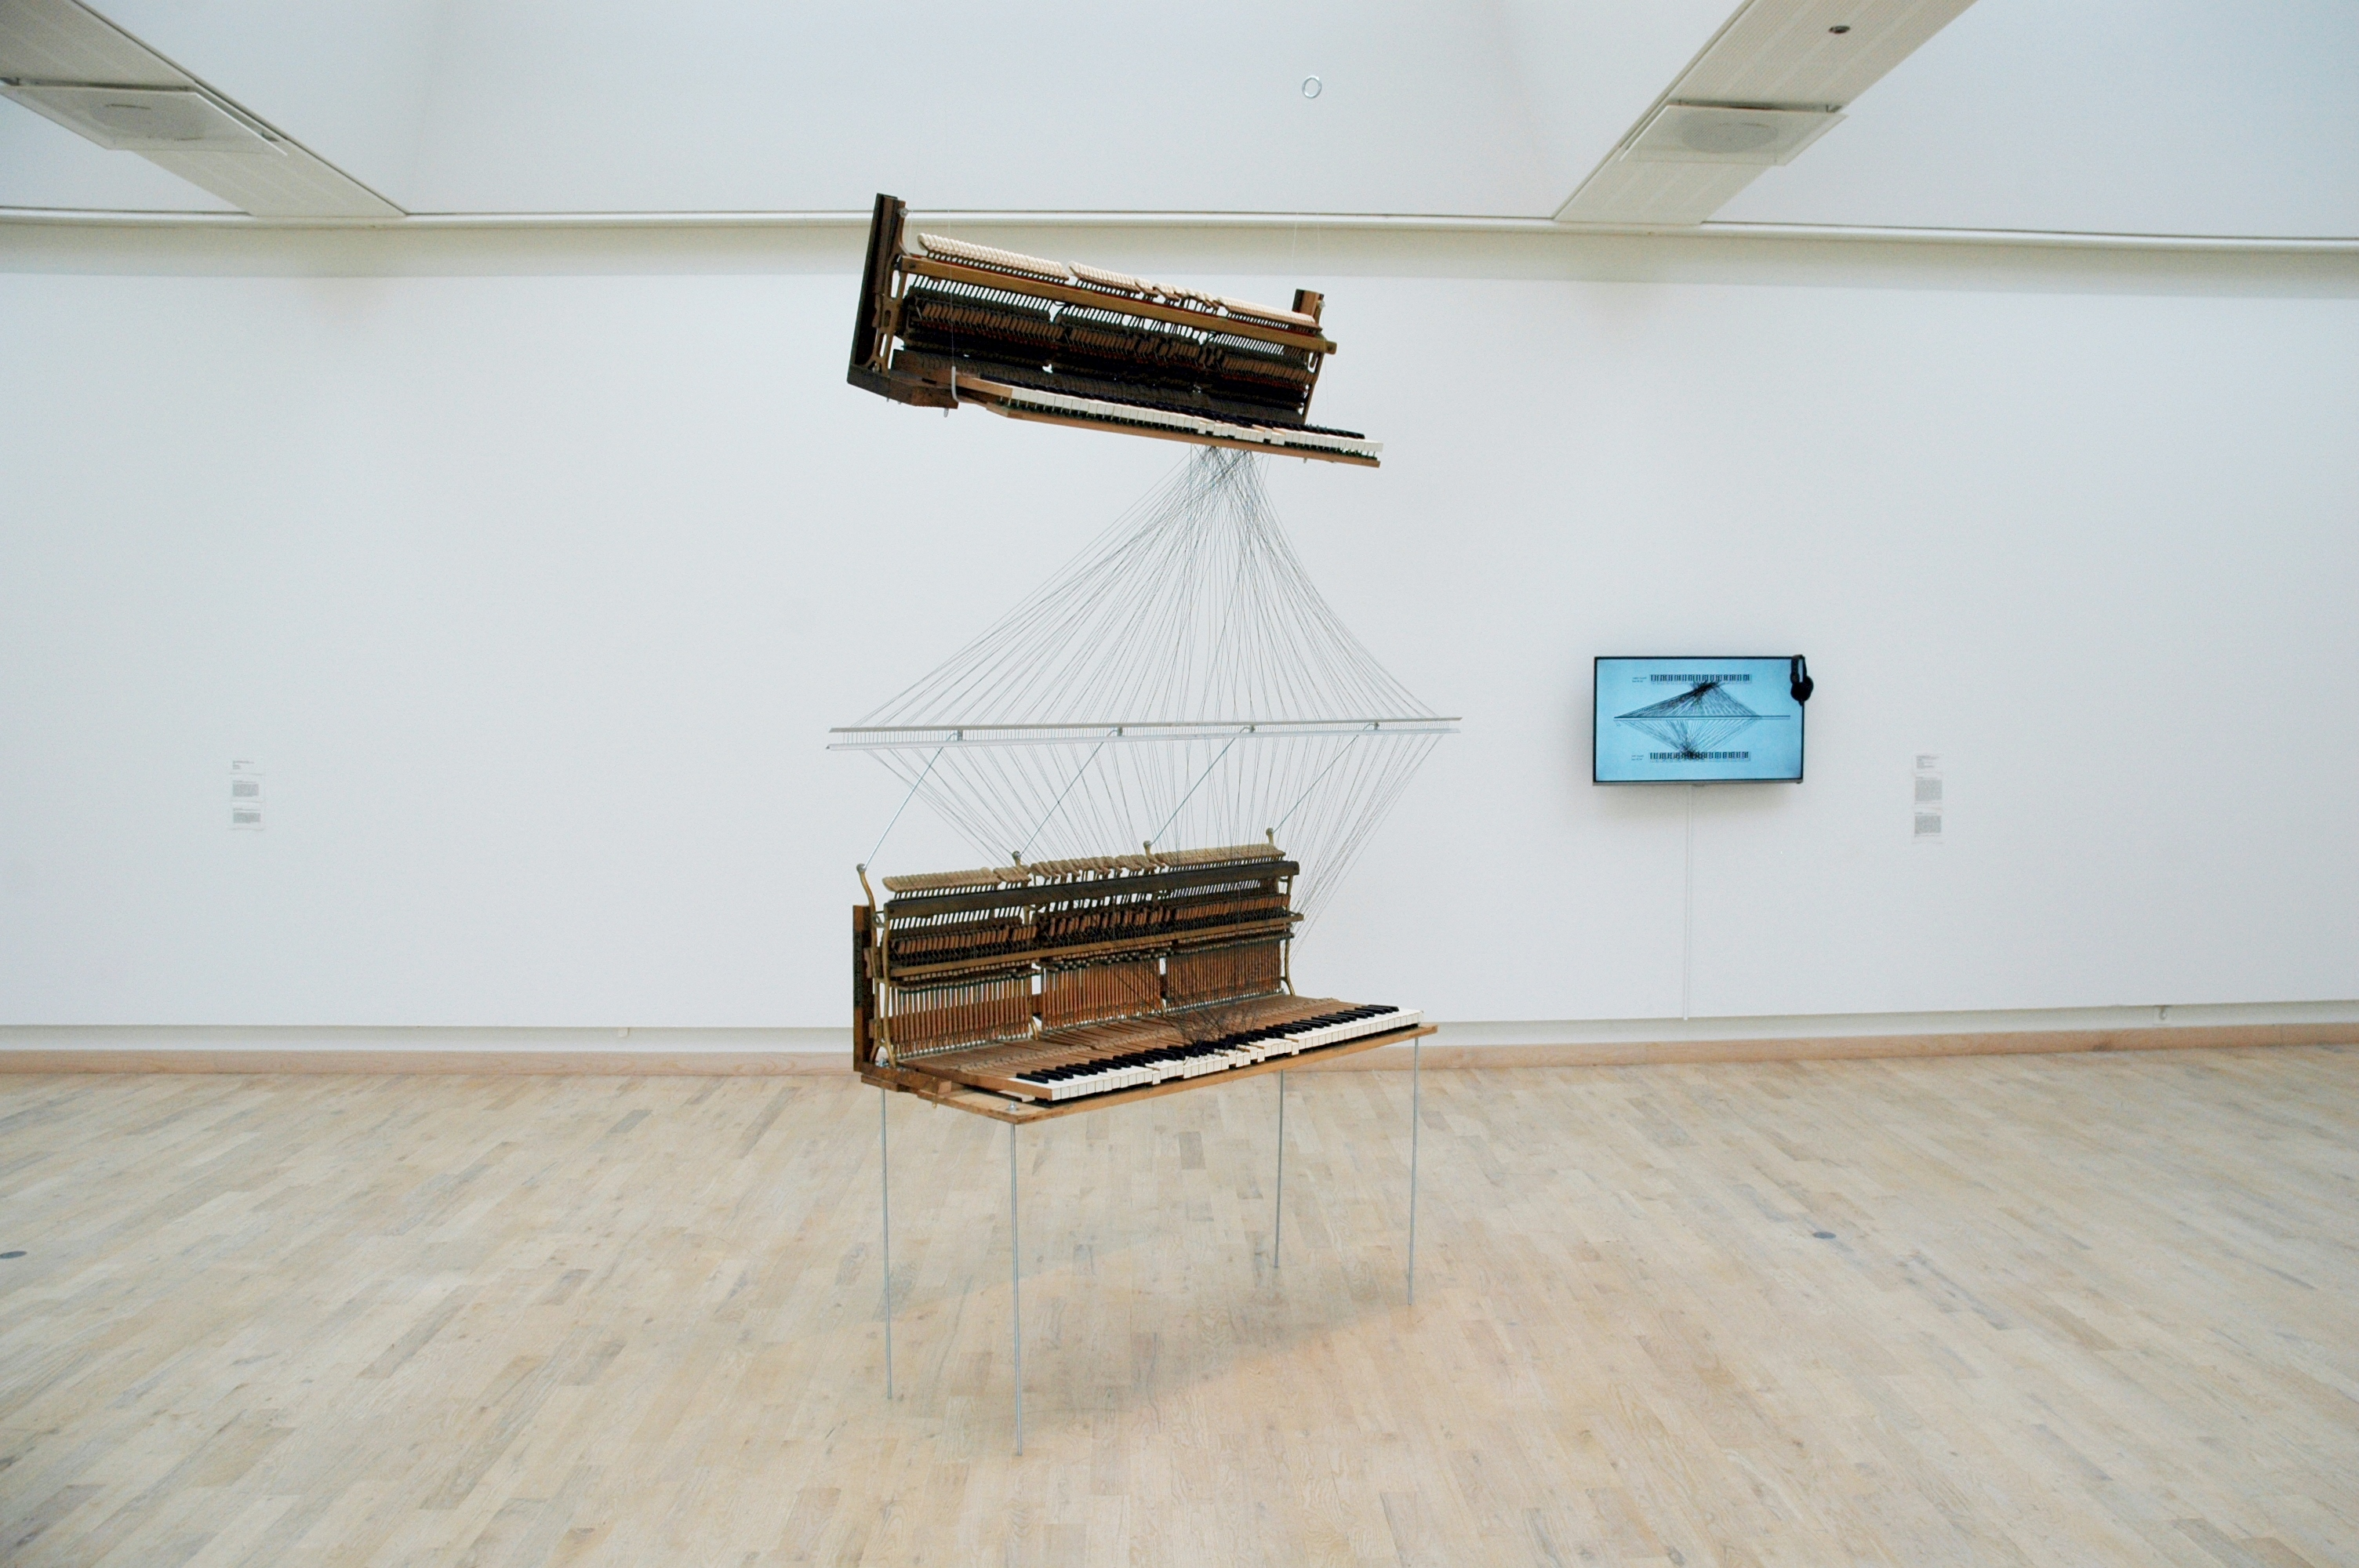
\includegraphics[width=\textwidth]{gfx/Einarson-SchumannSculpture}
	\caption{Einar Torfi Einarsson - Schumann-Sculpture (remnants + deracination)}
	\label{fig:gesture:einarsson}
\end{figure}


\iquote{Every music performance is a dramatic presentation for listeners and improvisers alike. In a sense, both groups play interactive roles as actors from their respective platforms. Just as the design of the hall, the stage and the lighting frames the band's activity for the audience's observation, it also frames the audience's activity for the band to observe. Performers and listeners form a communication loop in which the ction of each continuously affect the other.} Paul F. Berliner in \cite{berliner_thinking_2009}


%%%%%%%%%%%%%%%%%%%%
%-------------------------------------------
\subsection*{Dans les instruments numériques}


Les \glspl{DMI} ont souvent été analysés en tant qu'\gls{IHM}, et les conférences académiques qui leur sont consacré reflètent une culture dans laquelle l'interaction s'exprime via un cahier des charges préalablement identifié: une \gls{IHM} est utilisée dans le cas d'une tâche précise et sa qualité (ergonomie, précision, etc.) peut être mesurée de manière quantifiée.
Dans le cas des instruments de musique cependant, cette tâche est plus complexe, car les enjeux de la création musicale dépassent par essence tout objectif identifié et mesurable au préalable. Par ailleurs, les \glspl{DMI} sont destinés à plusieurs types "d'utilisateurs" ayant un rôle différent : le musicien qui joue de l'instrument, mais également le public, qui bien qu'il ne joue pas de l'instrument est amené à en observer la performance.

Low entry fee, high ceiling.

La performance musicale est un "jeu" qui comporte une part de duplicité. Le public d'un concert est toujours le sujet d'une illusion. 

Un des biais de la littérature sur l’affordance des instruments de musique numérique est qu’elle s’inspire souvent des objectifs de l’affordance des IHM en général, avec l’idée que l’instrument doit être compréhensible pour les “autres” utilisateurs potentiels que l’auteur de l’instrument. Pourtant, nombre d’instruments présentés dans la communauté NIME ne sont joués que par leurs auteurs (cf. [1], [2], [3]) et si le fait de vouloir transmettre son instrument aux autres est louable, il n’est pas gage de qualité en ce qui concerne la création qui sera faite avec cet instrument. 


L'art musical procède en partie de la magie et de l'illusion perceptive. Le musicien nous fait entendre des continuités (e.g. une mélodie) là où l'acoustique fait apparaitre une série discrète (e.g. des notes de piano), ou inversement des fissions (e.g. deux voix indépendantes) là où est jouée une série temporelle de notes sur un même instrument. (=> plutôt que des exemple entre parenthèse, mettre une figure illustrant fission e.g. Bach's Violin Partita No. 3, BWV 1006.)

Cette question du jeu entre le continu et le discret dépasse le seul cadre de la musique mais semble trouver dans cet art de nombreuses espaces d'expression.

Les théories de la perception, en particulier du Gestalt, viennent en partie expliquer les mécanismes qui pousse notre perception à créer des continuités où il n'en existe pas physiquement et inversement à catégoriser des événements selon certaines distances perceptives qui ne sont pas nécessairement en lien avec l'unité de source de production du son.

Si donc on analyse le geste musical, il faut nécessairement prendre en compte sa dimension subversive en ce qu'elle se traduit, particulièrement dans le cas des \glspl{DMI} et des productions musicales impliquant l'électronique en général, dans le design des instruments et outils qui servent à la créer.

\cite{bin_show_2018}

Une étude de Tsay \cite{tsay_sight_2013}, dans laquelle des amateurs et experts sont amenés à évaluer une performance musicale sur la seule base d'un enregistrement silencieux, met en évidence le rôle considérable du la part visuelle dans l'appréciation et l'évaluation de la performance.

Carte et guide , frettage adaptatif (cite \cite{goudard_playing_2014})


\iquote{De même, pour un violoniste, la manière dont il lève le bras et dont il va attaquer le son, la rapidité avec laquelle il prépare son coup d’archet nous renseignent un petit peu, mais pas complètement – parce que l’on ne sait pas quelle hauteur il va jouer – sur certaines catégories du son, comme le fait que le son sera agressif, fort, ou délicat et très doux. (...) Dans la musique instrumentale, cette causalité est très importante car cela participe de la façon dont nous la percevons et l’intérêt, avec la musique électronique, c’est que l’on peut remettre en question cette causalité-là : un tout petit geste peut provoquer une tempête. Entre le geste du pianiste qui va appuyer sur une touche du piano et le son qui va sortir, il y a une machine que j’appelle une boîte noire, qui peut inverser les polarités, c’est-à-dire que je peux très bien programmer la machine de manière à ce que plus le son qui va être joué va être minime, pianissimo, plus le son électronique qui va sortir va être au contraire démesuré : dans ce cas-là, le geste ne correspondra pas du tout au son.} Philippe Manoury interviewé par Anne-Sylvie Barthel-Calvet. (\url{https://geste.hypotheses.org/364})

Dans en Echo de Manoury, ce sont les formants de la voir qui contrôlent la partie électronique, c'est-à-dire un geste invisible, sans contact. (extensible au suivi de partition)


Pouvoir transformer tout type de donnée en geste programmé.


L'interface sensible\footnote{Sur la notion d'interface sensible, cf. \ref{ch:interfaces}} doit pouvoir se prêter à des gestes sans intention, c'est-à-dire qu'elle doit permettre des gestes non-réfléchi, mal-contrôlé ou plutôt in-controlés, qui peuvent tomber en dehors de la zone prévue pour capter de le geste, où d'une manière inadéquate. Cela ne signifie pas nécessairement que l'instrument doit ``faire quelque chose'' de ces gestes: il peut les ignorer.  Mais il est utile que l'intrument permette aux gestes de ``déborder'' du cadre prévu pour leur interaction (si toutefois ce cadre existe).


%-------------------------------------------
\subsection*{Tout ce qui bouge n'est pas geste - partie à revoir ou distribuer}

Dans le domaine de la recherche musicale, les mouvements du corps sont associés à la notion de \textit{geste musical}, c'est-à-dire à un concept associant à la fois le \textit{mouvement} du corps et \textit{l'intention} et/ou \textit{la signification} de ce mouvement. 

Cela n'est pas nécessairement et systématiquement le cas et les mouvements de l'instrumentiste peuvent être envisagés et décrits avec d'autres perspectives que celle de leur potentielle intention. \todo{ref ou footnote ici vers des études en ce sens} La notion de \textit{geste musical} semble en effet implicitement suggérer un rapport hiérarchique entre le musicien et son instrument, dans lequel les gestes ne serait produits qu'intentionnellement, à l'initiative du musicien. Les instruments de musique, et en particulier les DMIs, sont envisagés plus récemment comme \textit{agents} qui opèrent dans un système de relations multi-directionnelles\todo{ref}, que Berliner décrit métaphoriquement par une \textit{conversation} dans \cite{berliner_thinking_2009}. \todo{attention,il parle de la relation musicien/public} 

\Pierre{ je doute qu'il y ait beaucoup de gestes non-intentionnels chez le musicien !}


Les gestes du musicien ne sont pas nécessairement remplis d'une intention ou d'une signification \textit{a priori}, ils peuvent s'apparenter aux gestes de la danse.




L'instrument vibre et produit parfois du son sans qu'il soit explicitement déclenché ou controlé. Les mouvements du corps du musicien en témoignent et au dela des effets spectaculaires des DJs qui touchent aux potentiomètres de leurs interfaces comme s'ils étaient brûlants \footnote{Mark J. Butler apelle \iquote{passion of the knob} (\textit{la fièvre du potentiomètre}) ces moments qui surviennent \iquote{lorsqu'un musicien dirige une expressivité exceptionnellement intense vers un petit composante technique associée à l'ingénierie du son} \cite{butler_playing_2014} \url{https://www.youtube.com/watch?v=Nh9C7nQHmII}}, le corps est parcouru de mouvements qui ne sont pas uniquement des \textit{actions} mais des \textit{réactions} à ce qui est produit par l'instrument. 

\Pierre{ l'exemple choisi devrait être un peu plus analyser car les mouvements du DJs sont probablement totalement intentionnels - c-a-d ils font partie du spectacle car le DJ se sait regardé.}
\Pierre{ je crois plus en la séparation geste-signe et geste-action}

Si l'on considère la relation geste/instrument/musique comme un réseau multi-directionnel, le geste peut-être provoqué par la musique, via l'instrument lui même. Deux exemples caricaturaux viennent illuster cette possibilité : la performance \iquote{eletric stimulus to face — test} de l'artiste Daito Manabe\footnote{\url{http://www.daito.ws/work/electricstimulustoface_test.html}} ou dans le système de motorisation des doigts pour apprendre un instrument proposé récemment à la conférence NIME par \cite{zhang_adaptive_2019}.


Notons enfin que les mouvements peuvent survenir également en interaction avec le public\footnote{This reveals that passion-of-the-knob moments and other actions are not interior to the musician’s world, but rather are intensely meaningful communications: they reverberate outward to the audience and then are reflected back to the stage as formative elements of a milieu whose participants seek to actively cultivate and sustain liveness. in \cite{butler_playing_2014}} 



\subsection*{geste d'impression, geste d'expression}
Si le geste peut ex-primer, c'est-à-dire ``faire sortir en pressant'', un mouvement intérieur et le faire exister dans la temporalité de la performance, il peut aussi im-primer (faire rentrer, en pressant) ce geste sur un support à même d'en accueillir la trace.

geste du latin gero qui signifie ``porter''

S'il y a différance (ajournement et différence) dans la grammatisation musicale (la composition, la lutherie, la programmation), il y a enfin le moment de sa performance, de sa répétition.

Classification des controleurs gestuels dans \cite{wanderley_controgestuel_1999}:
\vspace{-1em}
\begin{itemize}[noitemsep]
\item \textbf{Instrument-like controllers},where the input device design tends to reproduce each feature of an existing (acoustic) instrument in detail. Many examples can be cited, such as electronic keyboards, guitars, saxophones, marimbas, and so on.
\item \textbf{Instrument-inspired controllers} that although largely inspired by the existing instrument’s design, are conceived for another use [62]. Fig. 3 presents one example of such controller, the SuperPolm violin developed by S. Goto, A. Terrier, and P. Pierrot [63], [64], where the input device is loosely based on a violin shape, but is used as a general device to control granular synthesis. => emprunts variés de formes et de fonctions.
\item \textbf{Extended instruments} are instruments augmented by the addition of extra sensors [58], [65]. Commercial augmented instruments included the Yamaha Disklavier, used, for instance, in pieces by J.-C. Risset[66], [67]. Other examples include the flute [68]–[70] and the trumpet [71]–[73], but any existing acoustic instrument may be extended to different degrees by the addition of sensors.
\item \textbf{Alternate controllers} (see, e.g., Fig. 4), whose design does not follow that of an established instrument. Some examples include the Hands [52], graphic drawing tablets [74] (cf. Fig. 5), etc. For instance, an unorthodox gestural controller using the shape of the oral cavity has been proposed in [75].
\end{itemize}

These controllers can furthermore be classified into different categories.
\begin{itemize}[noitemsep]
\item \textbf{Touch, expanded range, or immersive} controllers [76], depending on the amount of physical contact required from the performer. Mulder also [76] separates immersive controllers into internal, external, and symbolic controllers according to the possibilities of visualization of the control surface. In a different approach, Piringer [77] classifies immmersive controllers into partial or completely immersive controllers.
\item \textbf{Individual or collaborativecontrollers}[78],depending on whether the instrument is performed by one or multiple performers at one time.
\item \textbf{Metaphorical} or \item{ad hoc} controllers, and so on.
\end{itemize}


Guerino Mazzola frozen gestures



\iquote{Complétons tout d’abord la phrase : l’ordinateur n’est pas un instrument mais une représentation d’instrument. Cette subtile nuance contient l’essentiel. Envisagé ainsi, l’ordinateur donne une nouvelle dimension au processus de création en y intégrant explicitement, en amont de l’acte instrumental, la construction d’une représentation du dispositif instrumental. Cette construction\/représentation offre une latitude nouvelle : la possibilité pour l’homme de se placer dans une relation ``de type instrumental'', une représentation de relation instrumentale où la liberté d’échapper aux contingences du réel lui permet de créer de nouveaux mondes imaginaires. 
Toutefois, le processus de création est également considérablement transformé par le fait que l’aller\/retour indispensable entre le réel et l’imaginaire, lui aussi, se déplace. Dans le cas de l’instrument réel, l’aller\/retour se fait in situ, dans la relation même avec l’instrument. Dans le cas de la représentation d’instrument, il se fait dans une boucle plus vaste : l’activité de représentation instrumentale, de jeu virtuel, de composition façonnent nos sens et notre intelligence d’une nouvelle manière qui sont alors en jeu dans une perception nouvelle du monde réel... à condition que nous y retournions, c’est à dire que nous ne finissions pas par substituer définitivement nos représentations à la réalité.} \cite{cadoz_musique_1999}, p99.

Claude Cadoz défend l'hypothèse que les appareils électroniques ne sont pas des instruments mais des ``représentations d'instrument''.

L'apparence de causalité est fonction de
\vspace{-1em}
\begin{itemize}[noitemsep]
	\item congruence temporelle : synchronisation temporelle, morphologie rythmique similaire
	\item congruence spatiale : colocalisation spatiale, trajectoire similaires
	\item médiation par un objet intermédiaire dont on pense connaître le fonctionnement
\end{itemize}

